 % -*- TeX-engine: xetex; eval: (auto-fill-mode 0); eval: (visual-line-mode 1); -*-
% Compile with XeLaTeX

%%%%%%%%%%%%%%%%%%%%%%%
% Option 1: Slides: (comment for handouts)   %
%%%%%%%%%%%%%%%%%%%%%%%

%\documentclass[slidestop,compress,mathserif,12pt,t,professionalfonts,xcolor=table]{beamer}
%
%% solution stuff
%\newcommand{\solnMult}[1]{
%\only<1>{#1}
%\only<2->{\red{\textbf{#1}}}
%}
%\newcommand{\soln}[1]{\textit{#1}}

%%%%%%%%%%%%%%%%%%%%%%%
% Option 2: Slides: (to post)                          %
%%%%%%%%%%%%%%%%%%%%%%%
%
%\documentclass[slidestop,compress,mathserif,12pt,t,professionalfonts,xcolor=table]{beamer}
%
% % solution stuff
% \newcommand{\solnMult}[1]{#1}
% \newcommand{\soln}[1]{}

%%%%%%%%%%%%%%%%%%%%%%%%%%%%%%%
% Option 3: Handouts, without solutions (post before class)    %
%%%%%%%%%%%%%%%%%%%%%%%%%%%%%%%

% \documentclass[11pt,containsverbatim,handout,xcolor=xelatex,dvipsnames,table]{beamer}
%
% % handout layout
% \usepackage{pgfpages}
% \pgfpagesuselayout{4 on 1}[letterpaper,landscape,border shrink=5mm]
%
% % solution stuff
% \newcommand{\solnMult}[1]{#1}
% \newcommand{\soln}[1]{}

%%%%%%%%%%%%%%%%%%%%%%%%%%%%%%%%%%%%
% Option 4: Handouts, with solutions (may post after class if need be)    %
%%%%%%%%%%%%%%%%%%%%%%%%%%%%%%%%%%%%

 \documentclass[11pt,containsverbatim,handout,xcolor=xelatex,dvipsnames,table]{beamer}

 % handout layout
 \usepackage{pgfpages}
 \pgfpagesuselayout{4 on 1}[letterpaper,landscape,border shrink=5mm]

 % solution stuff
 \newcommand{\solnMult}[1]{\red{\textbf{#1}}}
 \newcommand{\soln}[1]{\textit{#1}}


%%%%%%%%%%
% Load style file, defaults  %
%%%%%%%%%%

%%%%%%%%%%%%%%%%
% Themes
%%%%%%%%%%%%%%%%

% See http://deic.uab.es/~iblanes/beamer_gallery/ for mor options

% Style theme
\usetheme{Pittsburgh}

% Color theme
\usecolortheme{seahorse}

% Helvetica Neue Light for most text
\usepackage{fontspec}
\setsansfont{Helvetica Neue Light}

%%%%%%%%%%%%%%%%
% Packages
%%%%%%%%%%%%%%%%

\usepackage{geometry}
\usepackage{graphicx}
\usepackage{amssymb}
\usepackage{epstopdf}
\usepackage{amsmath}  	% this permits text in eqnarray among other benefits
\usepackage{url}		% produces hyperlinks
\usepackage[english]{babel}
\usepackage{colortbl}	% allows for color usage in tables
\usepackage{multirow}	% allows for rows that span multiple rows in tables
\usepackage{color}		% this package has a variety of color options
\usepackage{pgf}
\usepackage{calc}
\usepackage{ulem}
\usepackage{multicol}
\usepackage{textcomp}
\usepackage{listings}
\usepackage{changepage}
\usepackage{tikz}
\usetikzlibrary{trees}		% for probability trees
\usepackage{fancyvrb}	% for colored code chunks
\usepackage{nameref}

%%%%%%%%%%%%%%%%
% Remove navigation symbols
%%%%%%%%%%%%%%%%

\beamertemplatenavigationsymbolsempty
\hypersetup{pdfpagemode=UseNone} % don't show bookmarks on initial view

%%%%%%%%%%%%%%%%
% User defined colors
%%%%%%%%%%%%%%%%

% Pantone 2015 Fall colors
% http://iwork3.us/2015/02/18/pantone-2015-fall-fashion-report/
% update each semester or year

\xdefinecolor{custom_blue}{rgb}{0, 0.32, 0.48} % FROM SPRING 2016 COLOR PREVIEW
\xdefinecolor{custom_darkBlue}{rgb}{0.20, 0.20, 0.39} % Reflecting Pond  
\xdefinecolor{custom_orange}{rgb}{0.96, 0.57, 0.42} % Cadmium Orange
\xdefinecolor{custom_green}{rgb}{0, 0.47, 0.52} % Biscay Bay
\xdefinecolor{custom_red}{rgb}{0.58, 0.32, 0.32} % Marsala

\xdefinecolor{custom_lightGray}{rgb}{0.78, 0.80, 0.80} % Glacier Gray
\xdefinecolor{custom_darkGray}{rgb}{0.35, 0.39, 0.43} % Stormy Weather

%%%%%%%%%%%%%%%%
% Template colors
%%%%%%%%%%%%%%%%

\setbeamercolor*{palette primary}{fg=white,bg= custom_blue}
\setbeamercolor*{palette secondary}{fg=black,bg= custom_blue!80!black}
\setbeamercolor*{palette tertiary}{fg=white,bg= custom_blue!80!black!80}
\setbeamercolor*{palette quaternary}{fg=white,bg= custom_blue}

\setbeamercolor{structure}{fg= custom_blue}
\setbeamercolor{frametitle}{bg= custom_blue!90}
\setbeamertemplate{blocks}[shadow=false]
\setbeamersize{text margin left=2em,text margin right=2em}

%%%%%%%%%%%%%%%%
% Styling fonts, bullets, etc.
%%%%%%%%%%%%%%%%

% title slide
\setbeamerfont{title}{size=\large,series=\bfseries}
\setbeamerfont{subtitle}{size=\large,series=\mdseries}
%\setbeamerfont{institute}{size=\large,series=\mdseries}

% color of alerted text
\setbeamercolor{alerted text}{fg=custom_orange}

% styling of itemize bullets
\setbeamercolor{item}{fg=custom_blue}
\setbeamertemplate{itemize item}{{{\small$\blacktriangleright$}}}
\setbeamercolor{subitem}{fg=custom_blue}
\setbeamertemplate{itemize subitem}{{\textendash}}
\setbeamerfont{itemize/enumerate subbody}{size=\footnotesize}
\setbeamerfont{itemize/enumerate subitem}{size=\footnotesize}

% styling of enumerate bullets
\setbeamertemplate{enumerate item}{\insertenumlabel.}
\setbeamerfont{enumerate item}{family={\fontspec{Helvetica Neue}}}
\setbeamerfont{enumerate subitem}{family={\fontspec{Helvetica Neue}}}
\setbeamerfont{enumerate subsubitem}{family={\fontspec{Helvetica Neue}}}

% make frame titles small to make room in the slide
\setbeamerfont{frametitle}{size=\small} 

% set Helvetica Neue font for frame and section titles
\setbeamerfont{frametitle}{family={\fontspec{Helvetica Neue}}}
\setbeamerfont{sectiontitle}{family={\fontspec{Helvetica Neue}}}
\setbeamerfont{section in toc}{family={\fontspec{Helvetica Neue}}}
\setbeamerfont{subsection in toc}{family={\fontspec{Helvetica Neue}}, size=\small}
\setbeamerfont{footline}{family={\fontspec{Helvetica Neue}}}
\setbeamerfont{subsection in toc}{family={\fontspec{Helvetica Neue}}}
\setbeamerfont{block title}{family={\fontspec{Helvetica Neue}}}

%%%%%%%%%%%%%%%%
% New fonts accessed by fontspec package
%%%%%%%%%%%%%%%%

% Monaco font for code
\newfontfamily{\monaco}{Monaco}

%%%%%%%%%%%%%%%%
% Color text commands
%%%%%%%%%%%%%%%%

%orange
\newcommand{\orange}[1]{\textit{\textcolor{custom_orange}{#1}}}

% yellow
\newcommand{\yellow}[1]{\textit{\textcolor{yellow}{#1}}}

% blue
\newcommand{\blue}[1]{\textit{\textcolor{blue}{#1}}}

% green
\newcommand{\green}[1]{\textit{\textcolor{custom_green}{#1}}}

% red
\newcommand{\red}[1]{\textit{\textcolor{custom_red}{#1}}}

% dark gray
\newcommand{\darkgray}[1]{\textit{\textcolor{custom_darkGray}{#1}}}

% light gray
\newcommand{\lightgray}[1]{\textit{\textcolor{custom_lightGray}{#1}}}

% pink
\newcommand{\pink}[1]{\textit{\textcolor{pink}{#1}}}


%%%%%%%%%%%%%%%%
% Custom commands
%%%%%%%%%%%%%%%%

% empty box for probability tree frame
\newcommand{\emptybox}[2]{
	\fbox{ \begin{minipage}{#1} \hfill\vspace{#2} \end{minipage} }
}

% cancel
\newcommand{\cancel}[1]{%
    \tikz[baseline=(tocancel.base)]{
        \node[inner sep=0pt,outer sep=0pt] (tocancel) {#1};
        \draw[red, line width=0.5mm] (tocancel.south west) -- (tocancel.north east);
    }%
}

% degree
\newcommand{\degree}{\ensuremath{^\circ}}

% cite
\newcommand{\ct}[1]{
\vfill
{\tiny #1}}

% Note
\newcommand{\Note}[1]{
\rule{2.5cm}{0.25pt} \\ \textit{\footnotesize{\textcolor{custom_red}{Note:} \textcolor{custom_darkGray}{#1}}}}

% Remember
\newcommand{\Remember}[1]{\textit{\scriptsize{\textcolor{custom_red}{Remember:} #1}}}

% links: webURL, webLink
\newcommand{\webURL}[1]{\urlstyle{same}{\textit{\textcolor{custom_blue}{\url{#1}}}}}
\newcommand{\webLink}[2]{\href{#1}{\textcolor{custom_blue}{{#2}}}}

% mail
\newcommand{\mail}[1]{\href{mailto:#1}{\textit{\textcolor{custom_blue}{#1}}}}

% highlighting: hl, hlGr, mathhl
\newcommand{\hl}[1]{\textit{\textcolor{custom_blue}{#1}}}
\newcommand{\hlGr}[1]{\textit{\textcolor{custom_green}{#1}}}
\newcommand{\mathhl}[1]{\textcolor{custom_blue}{\ensuremath{#1}}}

% example
\newcommand{\ex}[1]{\textcolor{blue}{{{\small (#1)}}}}

% two col: two columns
\newenvironment{twocol}[4]{
\begin{columns}[c]
\column{#1\textwidth}
#3
\column{#2\textwidth}
#4
\end{columns}
}

% slot (for probability calculations)
\newenvironment{slot}[2]{
\begin{array}{c} 
\underline{#1} \\ 
#2
\end{array}
}

% pr: left and right parentheses
\newcommand{\pr}[1]{
\left( #1 \right)
}

%%%%%%%%%%%%%%%%
% Custom blocks
%%%%%%%%%%%%%%%%

% activity: less commonly used
\newcommand{\activity}[2]{
\setbeamertemplate{itemize item}{{{\small\textcolor{custom_orange}{$\blacktriangleright$}}}}
\setbeamercolor{block title}{fg=white, bg=custom_orange}
\setbeamerfont{block title}{size=\small}
\setbeamercolor{block body}{fg=black, bg=custom_orange!20!white!80}
\setbeamerfont{block body}{size=\small}
\begin{block}{Activity: #1}
\setlength\abovedisplayskip{0pt}
#2
\end{block}
}

% app: application exercise
\newcommand{\app}[2]{
\setbeamercolor{block title}{fg=white,bg=custom_green}
\setbeamercolor{block body}{fg=black,bg=custom_green!20!white!80}
\begin{block}{{\small Application exercise: #1}}
#2
\end{block}
}

% disc: discussion question
\newcommand{\disc}[1]{
\vspace*{-2ex}
\setbeamercolor{block body}{bg=custom_blue!25!white!80, fg=custom_blue!55!black!95}
\begin{block}{\vspace*{-3ex}}
#1
\end{block}
\vspace*{-1ex}
}

% clicker: clicker question
\newcommand{\clicker}[1]{
\setbeamercolor{block title}{bg=custom_blue!80!white!50,fg=custom_blue!30!black!90}
\setbeamercolor{block body}{bg=custom_blue!20!white!80,fg=custom_blue!30!black!90}
\begin{block}{\vspace*{-0.2ex}{\footnotesize Clicker question}\vspace*{-0.2ex}}
#1
\end{block}
}

% formula
\newcommand{\formula}[2]{
\setbeamercolor{block title}{bg=custom_blue!40!white!60,fg=custom_blue!55!black!95}
\begin{block}{{\small#1}}
#2
\end{block}
}

% code
\newcommand{\Rcode}[1]{
{\monaco {\footnotesize \textcolor{custom_darkBlue}{#1}}}
}

% output
\newcommand{\Rout}[1]{
{\monaco {\footnotesize \textcolor{custom_darkGray}{#1}}}
}

%%%%%%%%%%%%%%%%
% Change margin
%%%%%%%%%%%%%%%%

\newenvironment{changemargin}[2]{%
\begin{list}{}{%
\setlength{\topsep}{0pt}%
\setlength{\leftmargin}{#1}%
\setlength{\rightmargin}{#2}%
\setlength{\listparindent}{\parindent}%
\setlength{\itemindent}{\parindent}%
\setlength{\parsep}{\parskip}%
}%
\item}{\end{list}}

%%%%%%%%%%%%%%%%
% Footnote
%%%%%%%%%%%%%%%%

\long\def\symbolfootnote[#1]#2{\begingroup%
\def\thefootnote{\fnsymbol{footnote}}\footnote[#1]{#2}\endgroup}

%%%%%%%%%%%%%%%%
% Graphics
%%%%%%%%%%%%%%%%

\DeclareGraphicsRule{.tif}{png}{.png}{`convert #1 `dirname #1`/`basename #1 .tif`.png}

%%%%%%%%%%%%%%%%
% Slide number
%%%%%%%%%%%%%%%%

\setbeamertemplate{footline}{%
    \raisebox{5pt}{\makebox[\paperwidth]{\hfill\makebox[20pt]{\color{gray}
          \scriptsize\insertframenumber}}}\hspace*{5pt}}

          
%%%%%%%%%%%%%%%%
% Remove page numbers
%%%%%%%%%%%%%%%%

\newcommand{\removepagenumbers}{% 
  \setbeamertemplate{footline}{}
}

%%%%%%%%%%%%%%%%
% TOC slides
%%%%%%%%%%%%%%%%

\setbeamertemplate{section in toc}{\inserttocsectionnumber.~\inserttocsection}
\setbeamertemplate{subsection in toc}{$\qquad$\inserttocsubsectionnumber.~\inserttocsubsection \\}

\AtBeginSection[] 
{ 
  \addtocounter{framenumber}{-1} 
  % 
  {\removepagenumbers 
  {\small
    \begin{frame}<beamer> 
    \frametitle{Outline} 
    \tableofcontents[currentsection] 
  \end{frame} 
  } 
  }
} 

\AtBeginSubsection[] 
{ 
  \addtocounter{framenumber}{-1} 
  % 
  {\removepagenumbers 
  {\small
    \begin{frame}<beamer> 
    \frametitle{Outline} 
    \tableofcontents[currentsection,currentsubsection] 
  \end{frame} 
  } 
  }
}
% You cannot use numbers when defining variables.  
% Hence the use of letters, A, B, C, etc.

% Course Name
\newcommand{\CourseName}{Sta 101 - Fall 2015}
\newcommand{\InstituteName}{Duke University, Department of Statistical Science}

% Personal Info
\newcommand{\FirstName}{Mine}
\newcommand{\LastName}{\c{C}etinkaya-Rundel}
\newcommand{\OfficeHours}{Tue + Thur 4:30-6pm}
\newcommand{\OfficeHoursLocation}{Old Chem 213}

% Electronic Info
\newcommand{\PersonalSite}{http://stat.duke.edu/~mc301}
\newcommand{\CourseSite}{http://bit.ly/sta101_f15}
\newcommand{\Email}{mine@stat.duke.edu}

% TAs
\newcommand{\TAA}{Erika Ball}
\newcommand{\TAB}{David Clancy}
\newcommand{\TAC}{Reuben McCreanor}
\newcommand{\TAD}{Anne Driscoll}
\newcommand{\TAE}{Megan Robertson}

% Exam Dates
\newcommand{\ExamADate}{Mon, Oct 5}
\newcommand{\ExamBDate}{Mon, Nov 9}
\newcommand{\FinalDate}{Thur, Dec 10 (2-5pm)}


% ALT ALT
% % You cannot use numbers when defining variables.  
% Hence the use of letters, A, B, C, etc.

% Personal Info
\newcommand{\FirstName}{Anthea}
\newcommand{\LastName}{Monod}
\newcommand{\OfficeHours}{TBA}
\newcommand{\OfficeHoursLocation}{TBA}

% Electronic Info
\newcommand{\PersonalSite}{TBA}
\newcommand{\CourseSite}{TBA}
\newcommand{\Email}{TBA}

% TAs
\newcommand{\TAA}{TBA}
\newcommand{\TAB}{TBA}
\newcommand{\TAC}{TBA}
\newcommand{\TAD}{TBA}
\newcommand{\TAE}{TBA}

% Exam Dates
\newcommand{\ExamADate}{TBA}
\newcommand{\ExamBDate}{TBA}
\newcommand{\FinalDate}{TBA}



%%%%%%%%%%%
% Cover slide info    %
%%%%%%%%%%%

\title{Unit 5: Inference for categorical data}
\subtitle{4. MT2 Review}
\author{\CourseName}
\date{}
\institute{\InstituteName}


%%%%%%%%%%%%%%%%%%%%%%%%%
% Begin document and set Helvetica Neue font   %
%%%%%%%%%%%%%%%%%%%%%%%%%

\begin{document}
\fontspec[Ligatures=TeX]{Helvetica Neue Light}

%%%%%%%%%%%%%%%%%%%%%%%%%%%%%%%%%%%

% Title Page

\begin{frame}[plain]

\titlepage

\vfill

{\scriptsize \webLink{\PersonalSite}{Dr. \LastName{}} \hfill Slides posted at  \webURL{\CourseSite}}

\addtocounter{framenumber}{-1} 

\end{frame}

%%%%%%%%%%%%%%%%%%%%%%%%%%%%%%%%%%%%

\section{Housekeeping}

%%%%%%%%%%%%%%%%%%%%%%%%%%%%%%%%%%%%

\begin{frame}
\frametitle{Announcements}

\begin{itemize}

\item MT 2 next week
\begin{itemize}
\item Bring a calculator + cheat sheet + writing utensil
\item Tables will be provided
\end{itemize}

\item MT 2 review session: Sat, Nov 7, 4-5pm, Old Chem 116
\begin{itemize}
\item[+] office hours as usual: \webURL{https://stat.duke.edu/courses/Fall15/sta101.002/info/\#oh}
\item[+] extra office hours from Dr. Monod: Friday, 1:30-3pm (Old Chem 122A)
\end{itemize}

\item MT 2 review materials posted on the course website

\item Project 1 due Friday evening (+ work on it in lab on Thursday)

\item PS 5 due Friday evening, PA 5 due Saturday evening (note day change to allow for review before midterm)

\end{itemize}

\end{frame}

%%%%%%%%%%%%%%%%%%%%%%%%%%%%%%%%%%%%

\section{Map of concepts}

%%%%%%%%%%%%%%%%%%%%%%%%%%%%%%%%%%%%

\begin{frame}

\vfill

\begin{center}
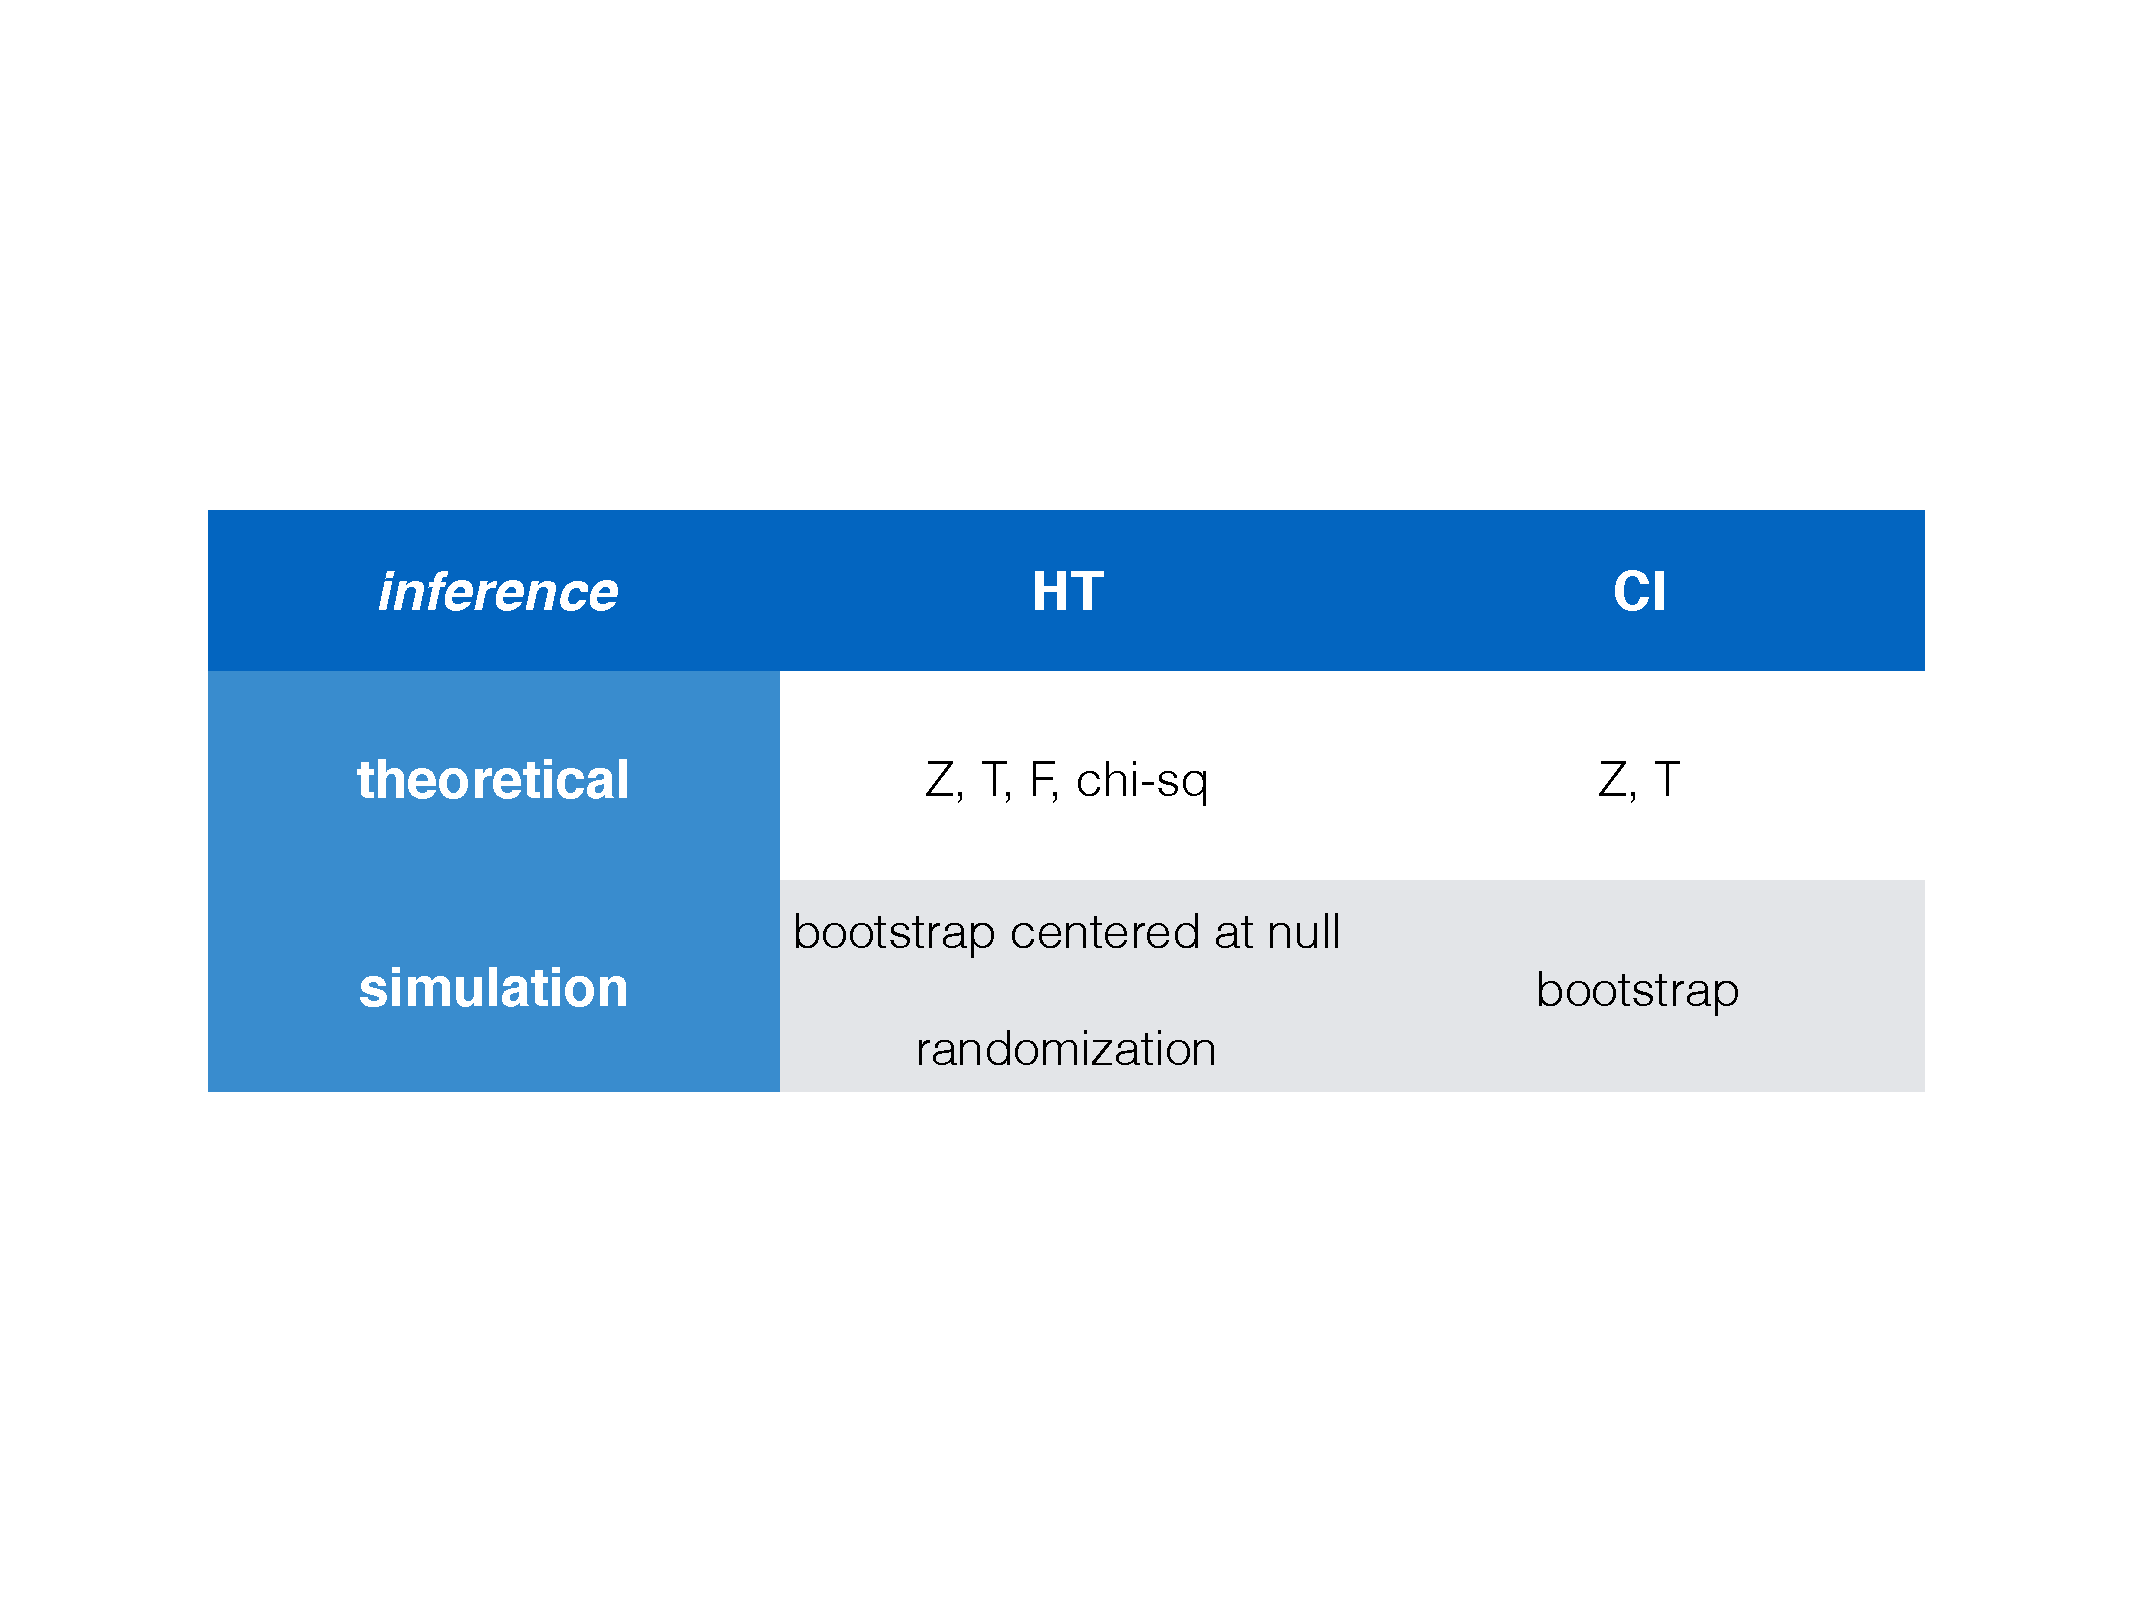
\includegraphics[width=\textwidth]{figures/mt2_review_map1}
\end{center}

\vfill

\end{frame}

%%%%%%%%%%%%%%%%%%%%%%%%%%%%%%%%%%%%

\begin{frame}

\begin{center}
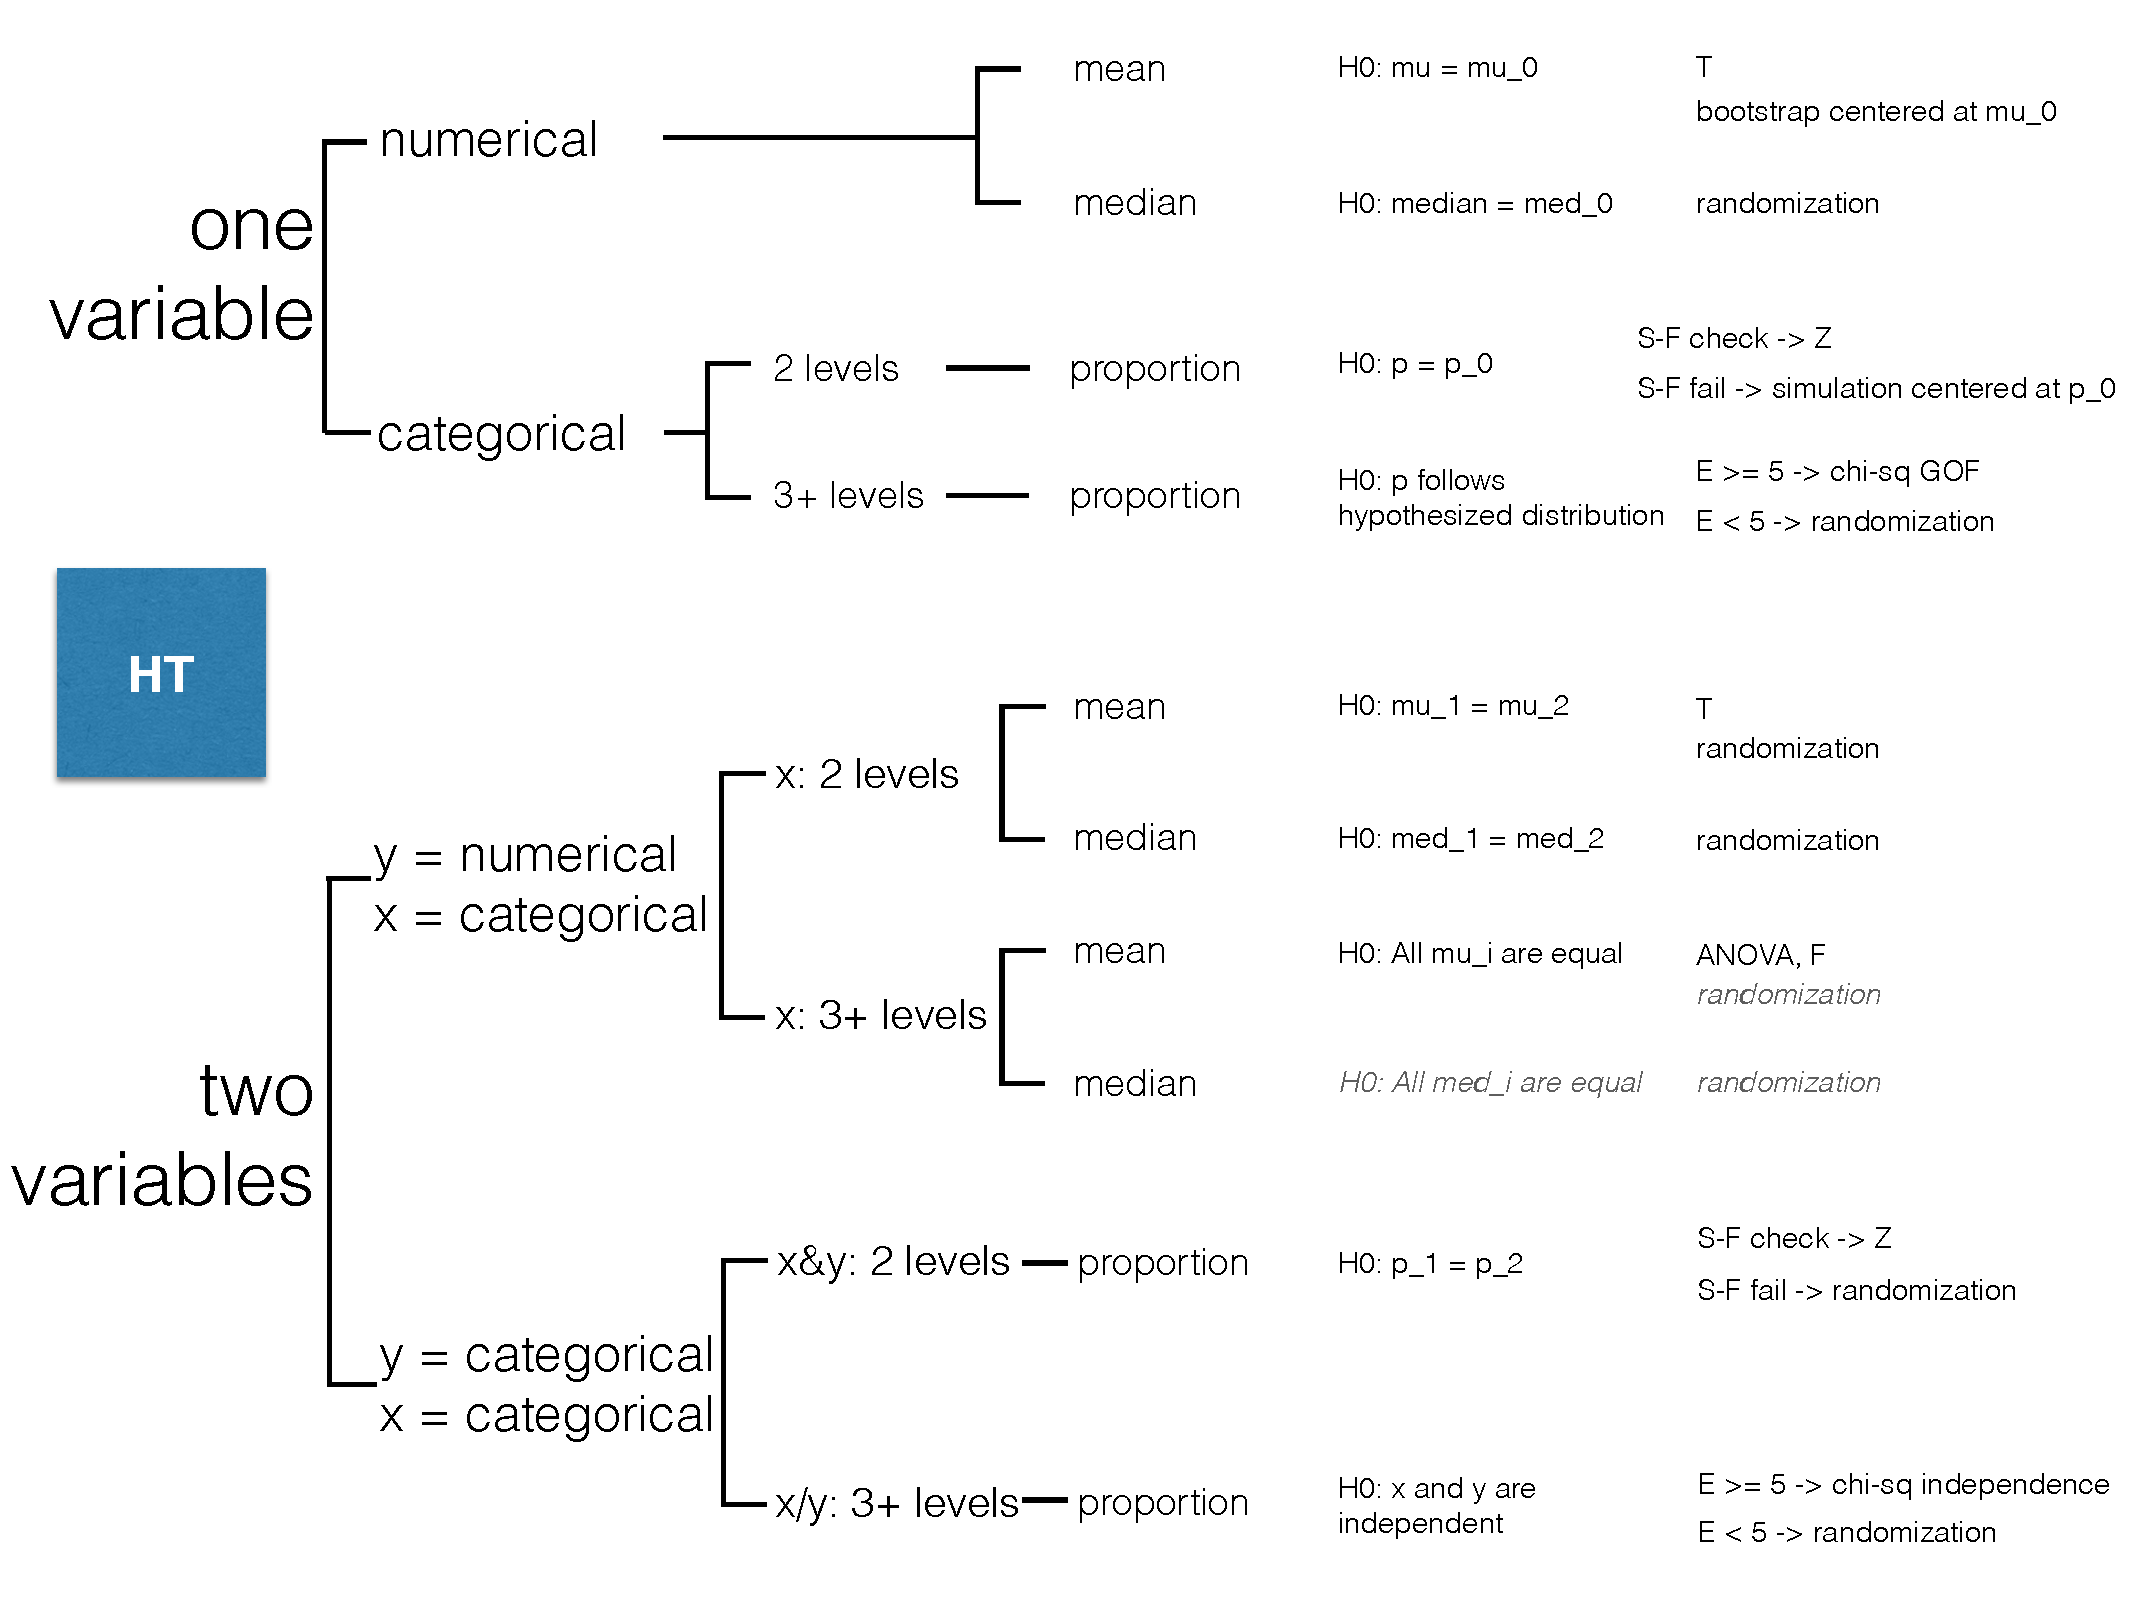
\includegraphics[width=\textwidth]{figures/mt2_review_map2}
\end{center}

\end{frame}

%%%%%%%%%%%%%%%%%%%%%%%%%%%%%%%%%%%%

\begin{frame}

\begin{center}
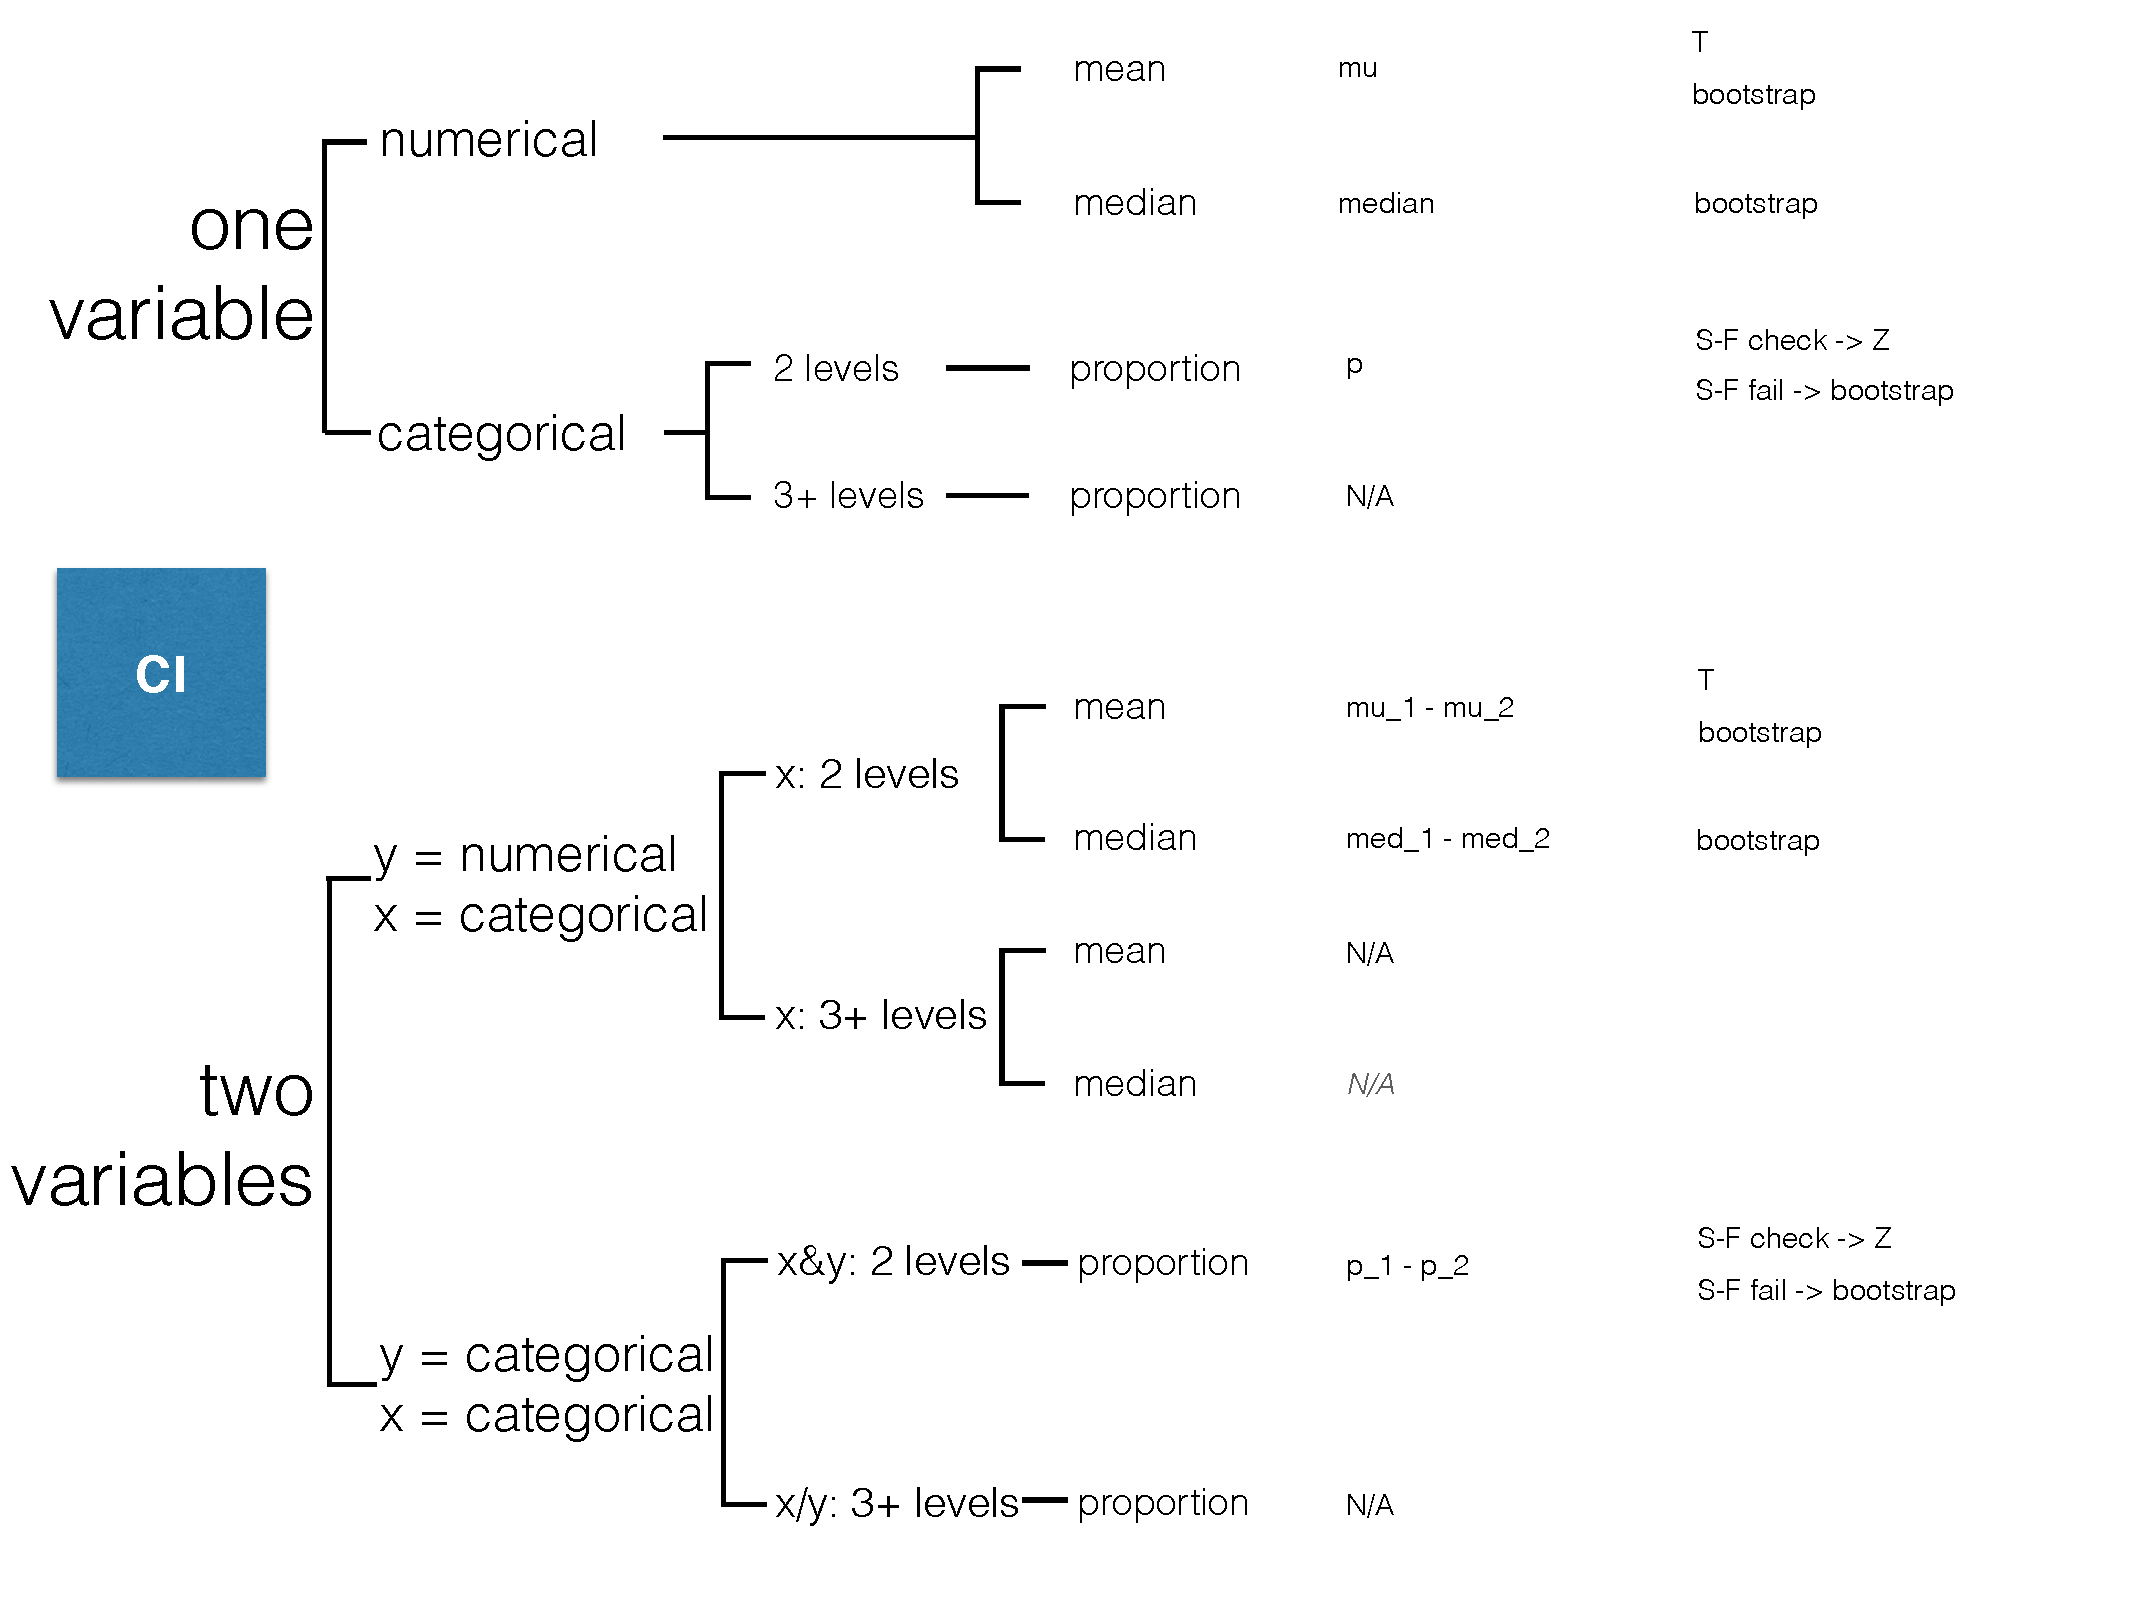
\includegraphics[width=\textwidth]{figures/mt2_review_map3}
\end{center}

\end{frame}

%%%%%%%%%%%%%%%%%%%%%%%%%%%%%%%%%%%%

\section{Review exercises}

%%%%%%%%%%%%%%%%%%%%%%%%%%%%%%%%%%%%

\begin{frame}

\twocol{0.7}{0.3}
{
{\scriptsize
\clicker{Which of the following is \underline{true}?
}}}
{
 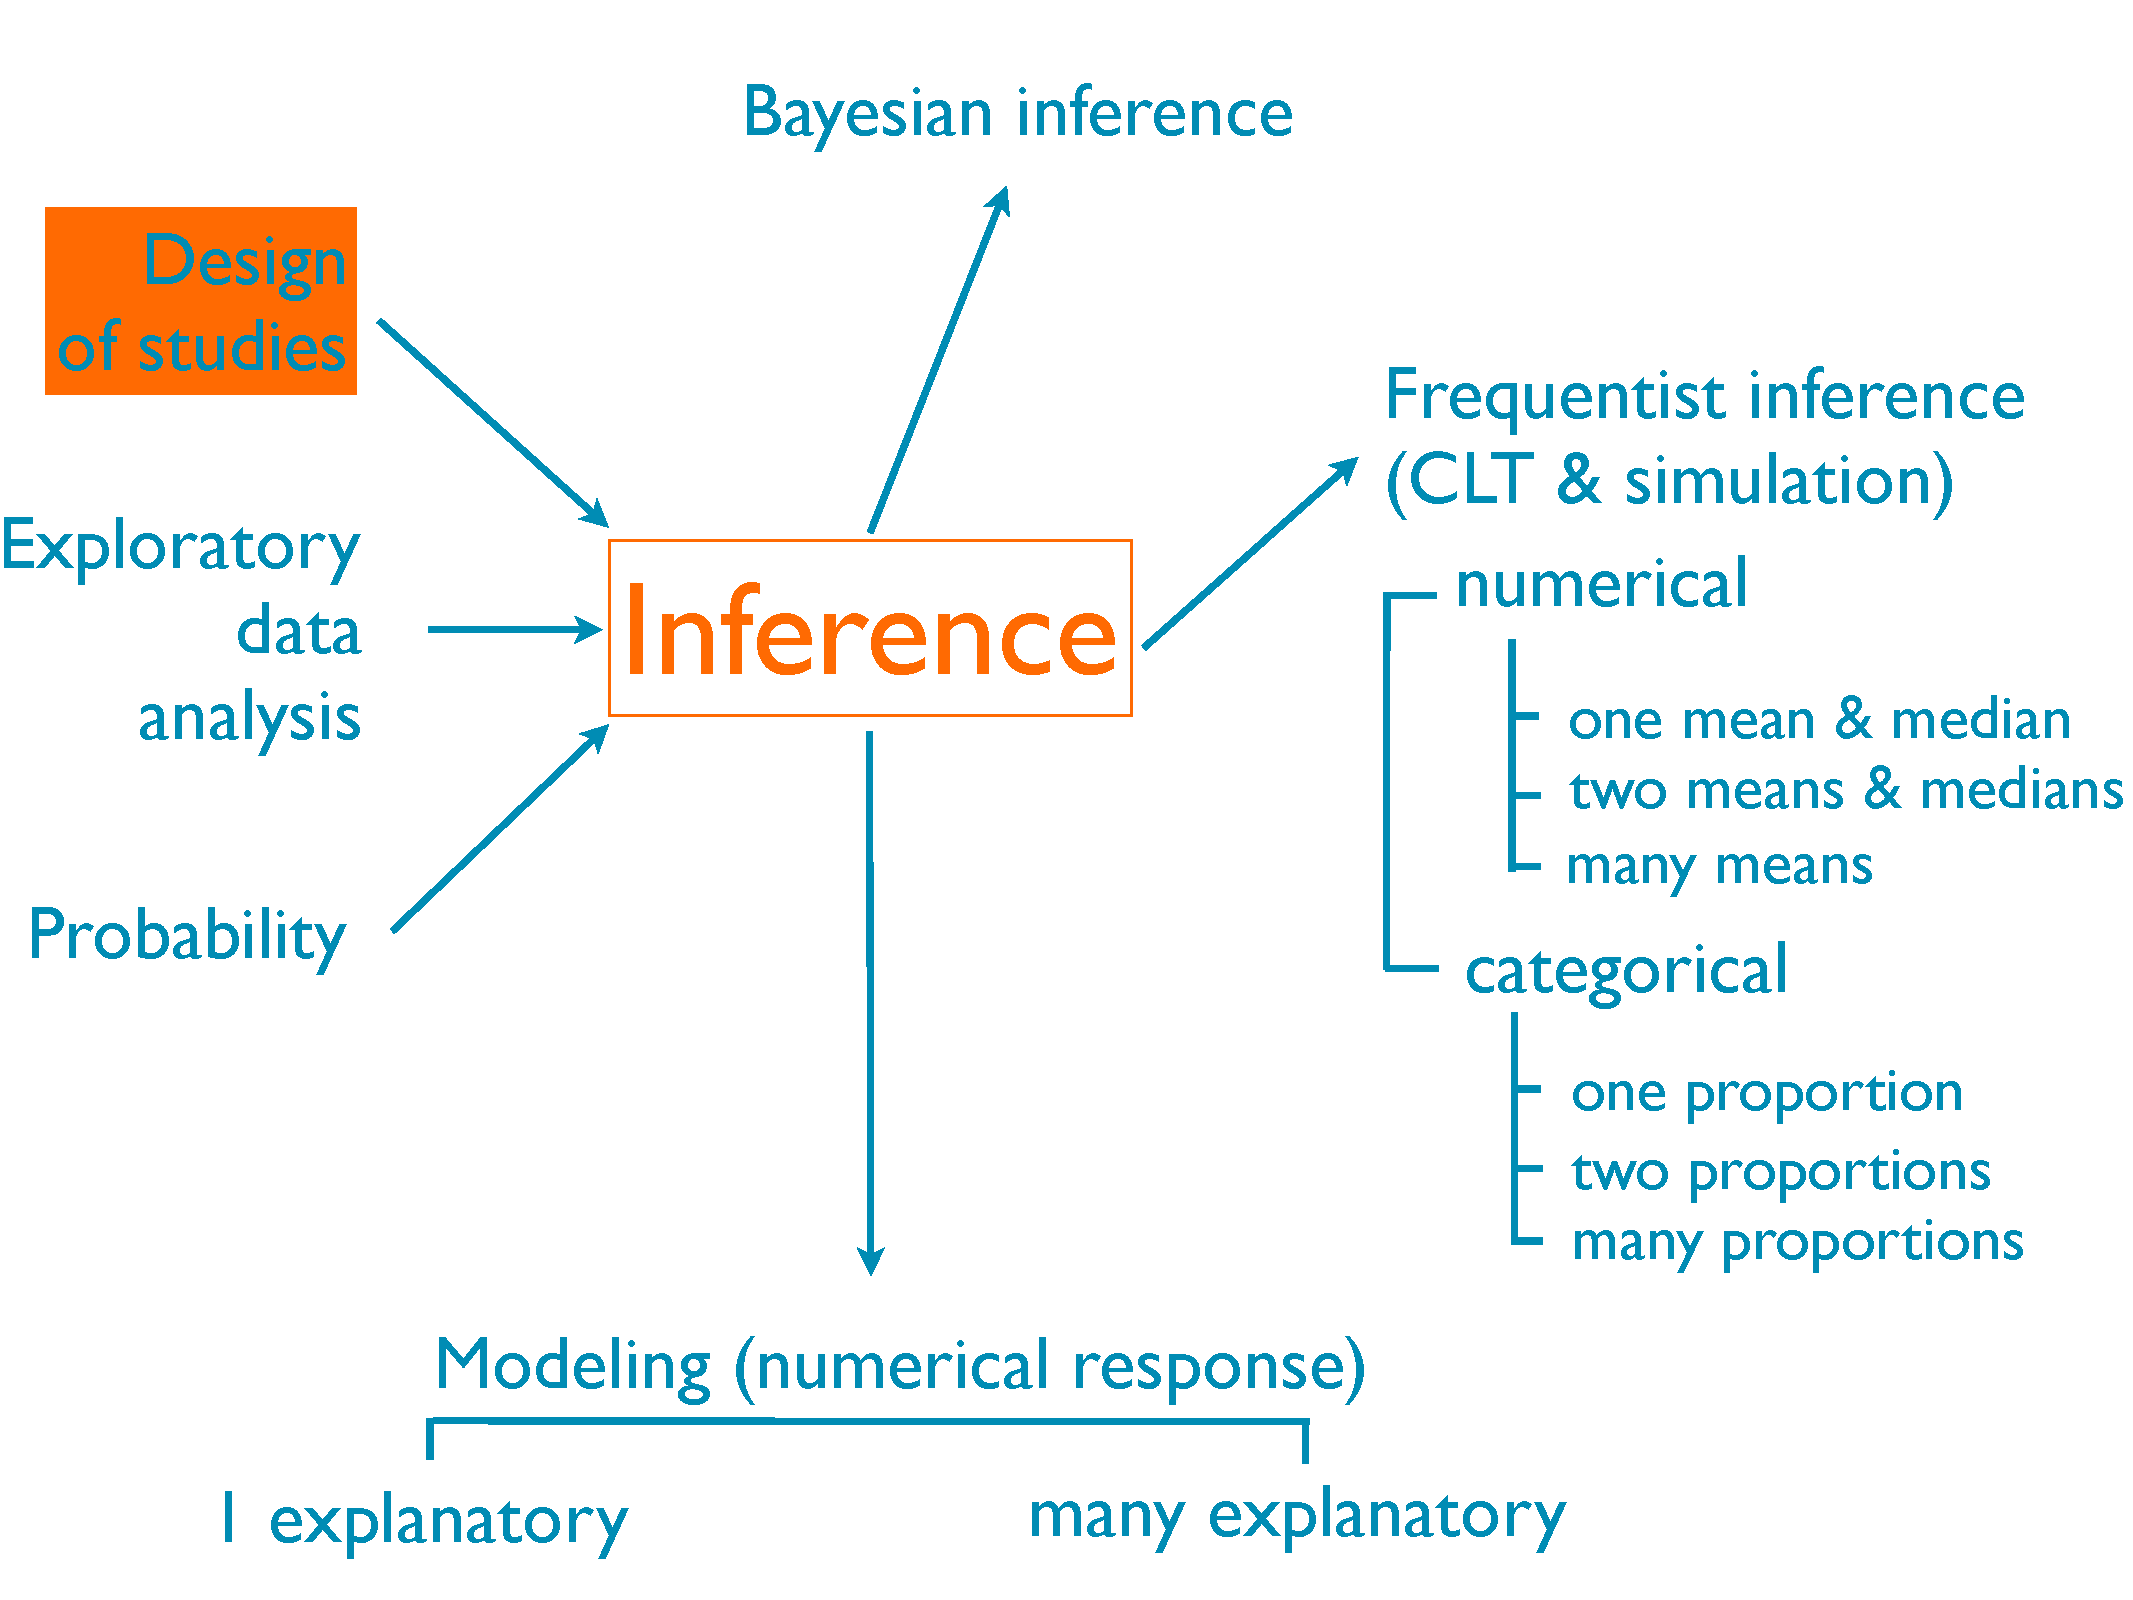
\includegraphics[width=\textwidth]{figures/map/design}
}

\vfill

{\footnotesize
\begin{enumerate}[(a)]
\item If the sample size is large enough, conclusions can be generalized to the population.
\item If subjects are randomly assigned to treatments, conclusions can be generalized to the population.
\item \solnMult{Blocking in experiments serves a similar purpose as stratifying in observational studies.}
\item Representative samples allow us to make causal conclusions.
\item Statistical inference requires normal distribution of the response variable.
\end{enumerate}
}

\end{frame}

%%%%%%%%%%%%%%%%%%%%%%%%%%%%%%%%%%%%

\begin{frame}

\twocol{0.7}{0.3}
{
{\scriptsize
\clicker{Which of the following is the best visualization for evaluating the relationship between two categorical variables?
}}}
{
 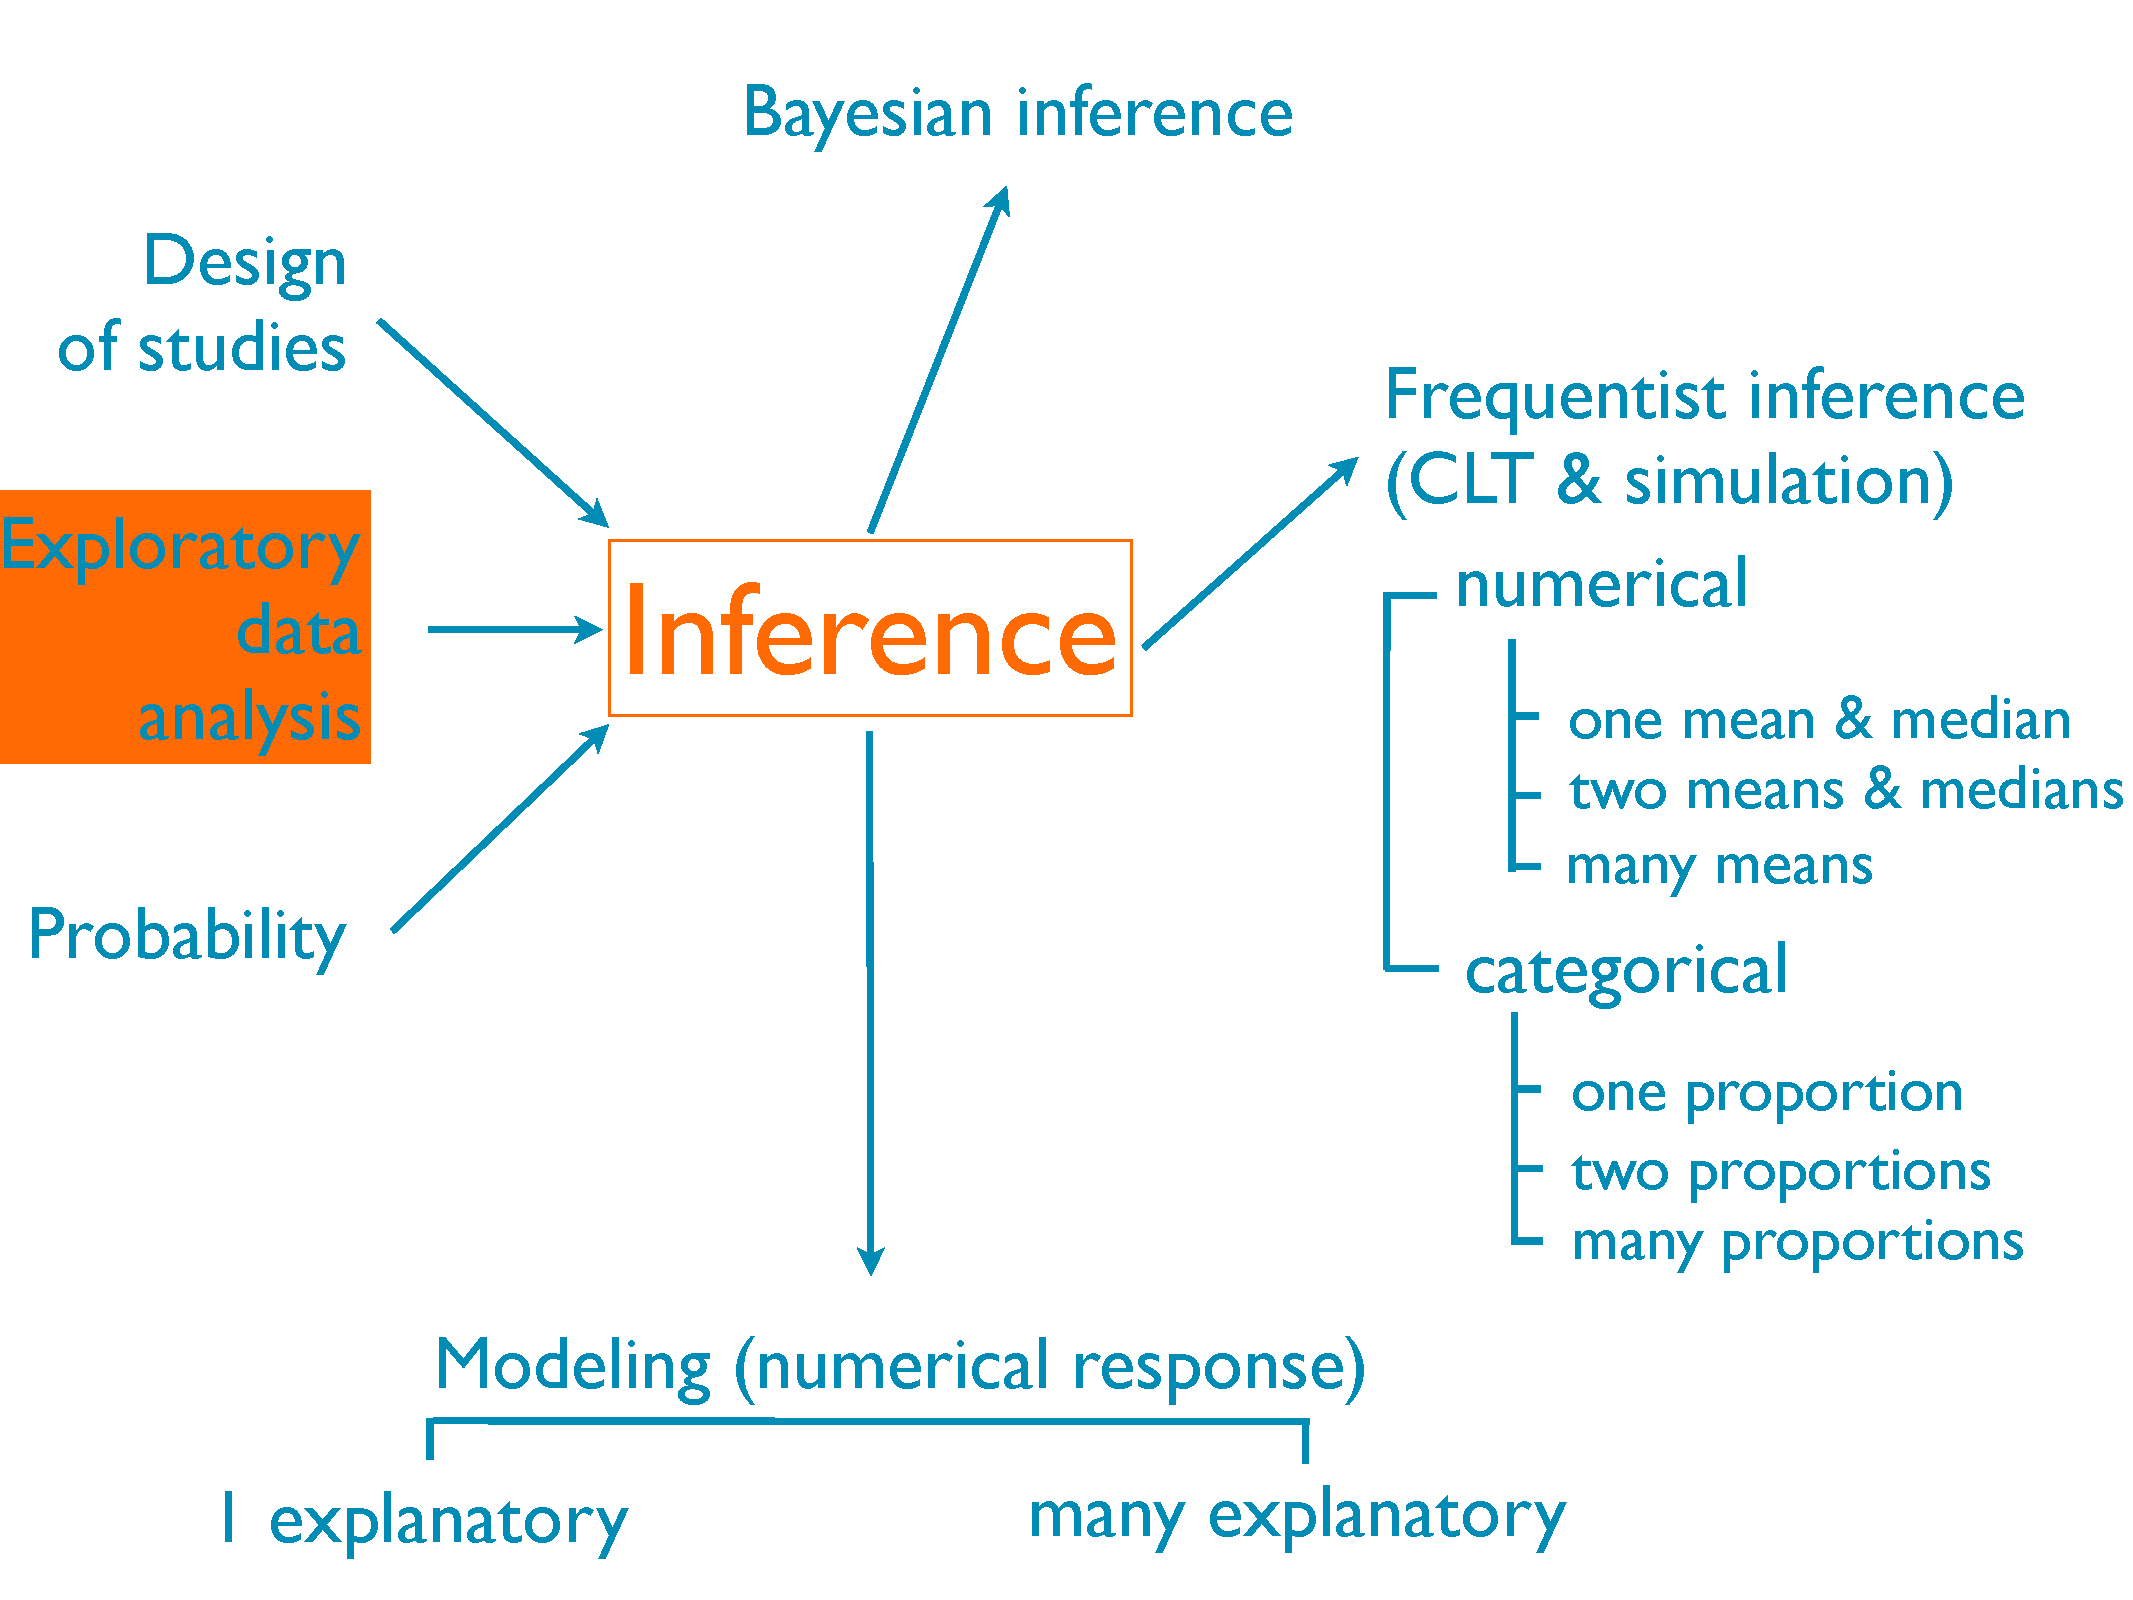
\includegraphics[width=\textwidth]{figures/map/eda}
}

\vfill

{\footnotesize
\begin{enumerate}[(a)]
\item side-by-side box plots
\item \solnMult{mosaic plot}
\item pie chart
\item segmented frequency bar plot
\item relative frequency histogram
\end{enumerate}
}

\end{frame}

%%%%%%%%%%%%%%%%%%%%%%%%%%%%%%%%%%%%

\begin{frame}

\twocol{0.7}{0.3}
{
{\scriptsize
\clicker{Two students in an introductory statistics class choose to conduct similar studies estimating the proportion of smokers at their school. Student A collects data from 100 students, and student B collects data from 50 students. How will the standard errors used by the two students compare? Assume both are simple random samples.}}}
{
 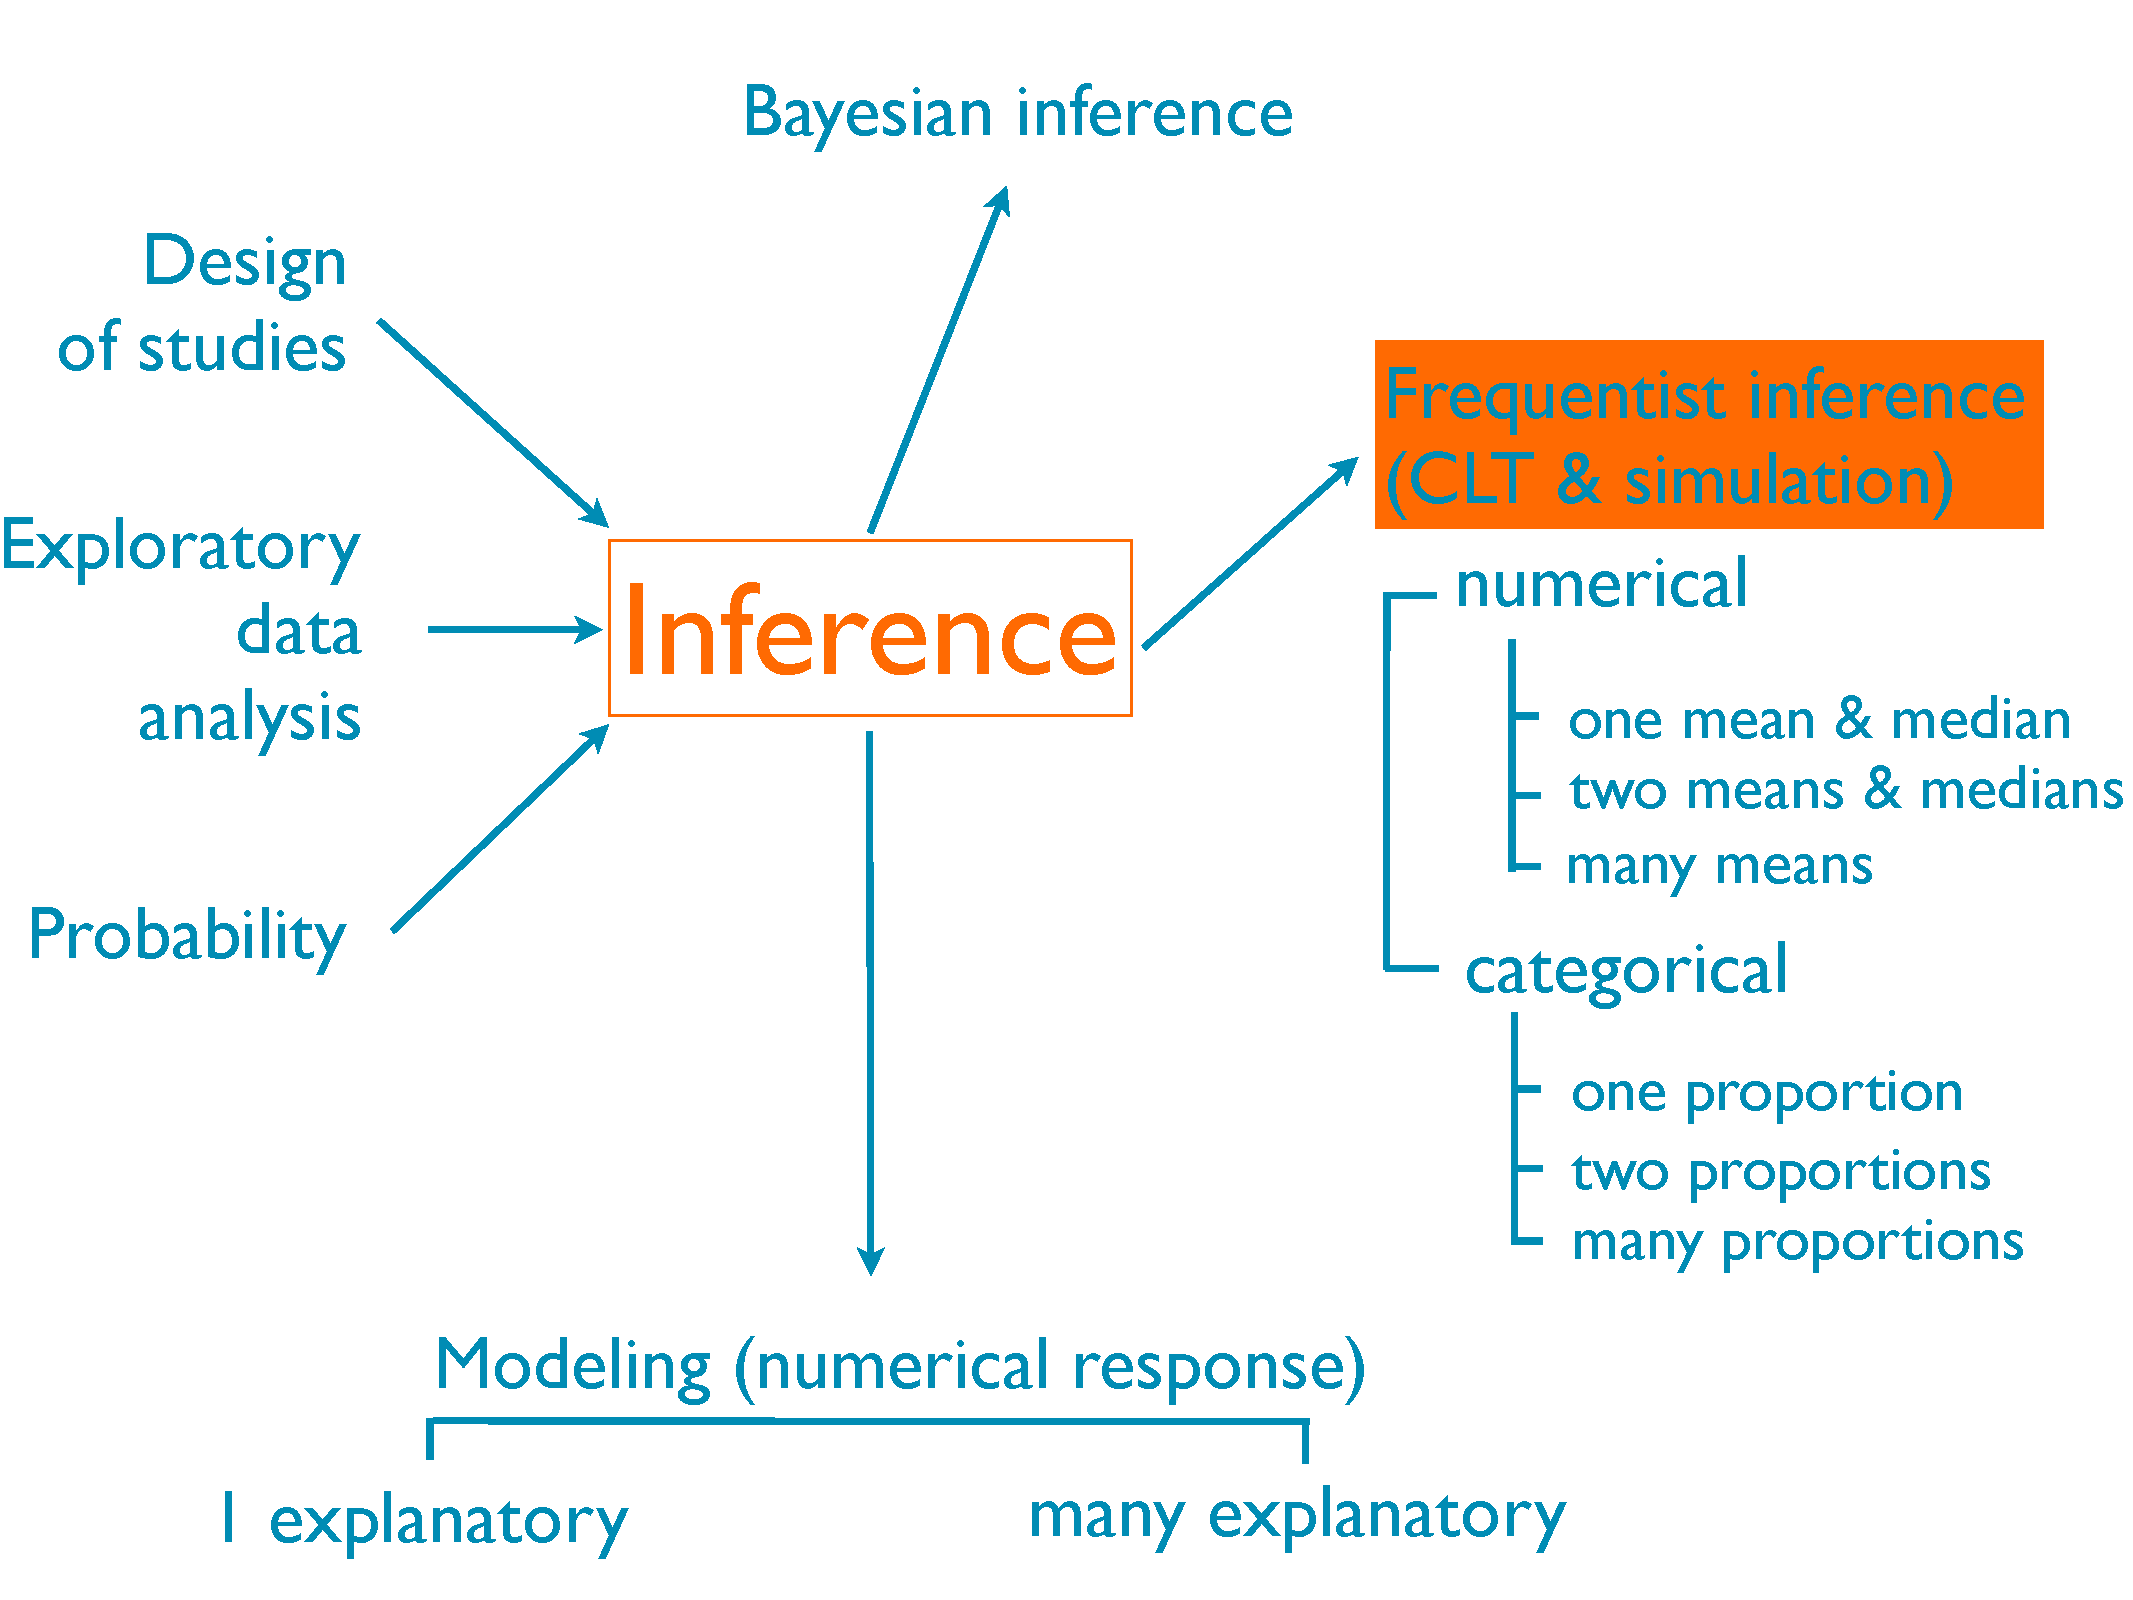
\includegraphics[width=\textwidth]{figures/map/clt}
}

\begin{enumerate}[(a)]
\item \solnMult{SE used by Student A $<$ SE used as Student B.}
\item SE used by Student A $>$ SE used as Student B.
\item SE used by Student A $=$ SE used as Student B.
\item SE used by Student A $\approx$ SE used as Student B.
\item Cannot tell without knowing the true proportion of smokers at this school.
\end{enumerate}

\end{frame}

%%%%%%%%%%%%%%%%%%%%%%%%%%%%%%%%%%%%

\begin{frame}

\twocol{0.7}{0.3}
{
{\scriptsize
\clicker{Which of the following is the best method for evaluating the relationship between two categorical variables?}}}
{
 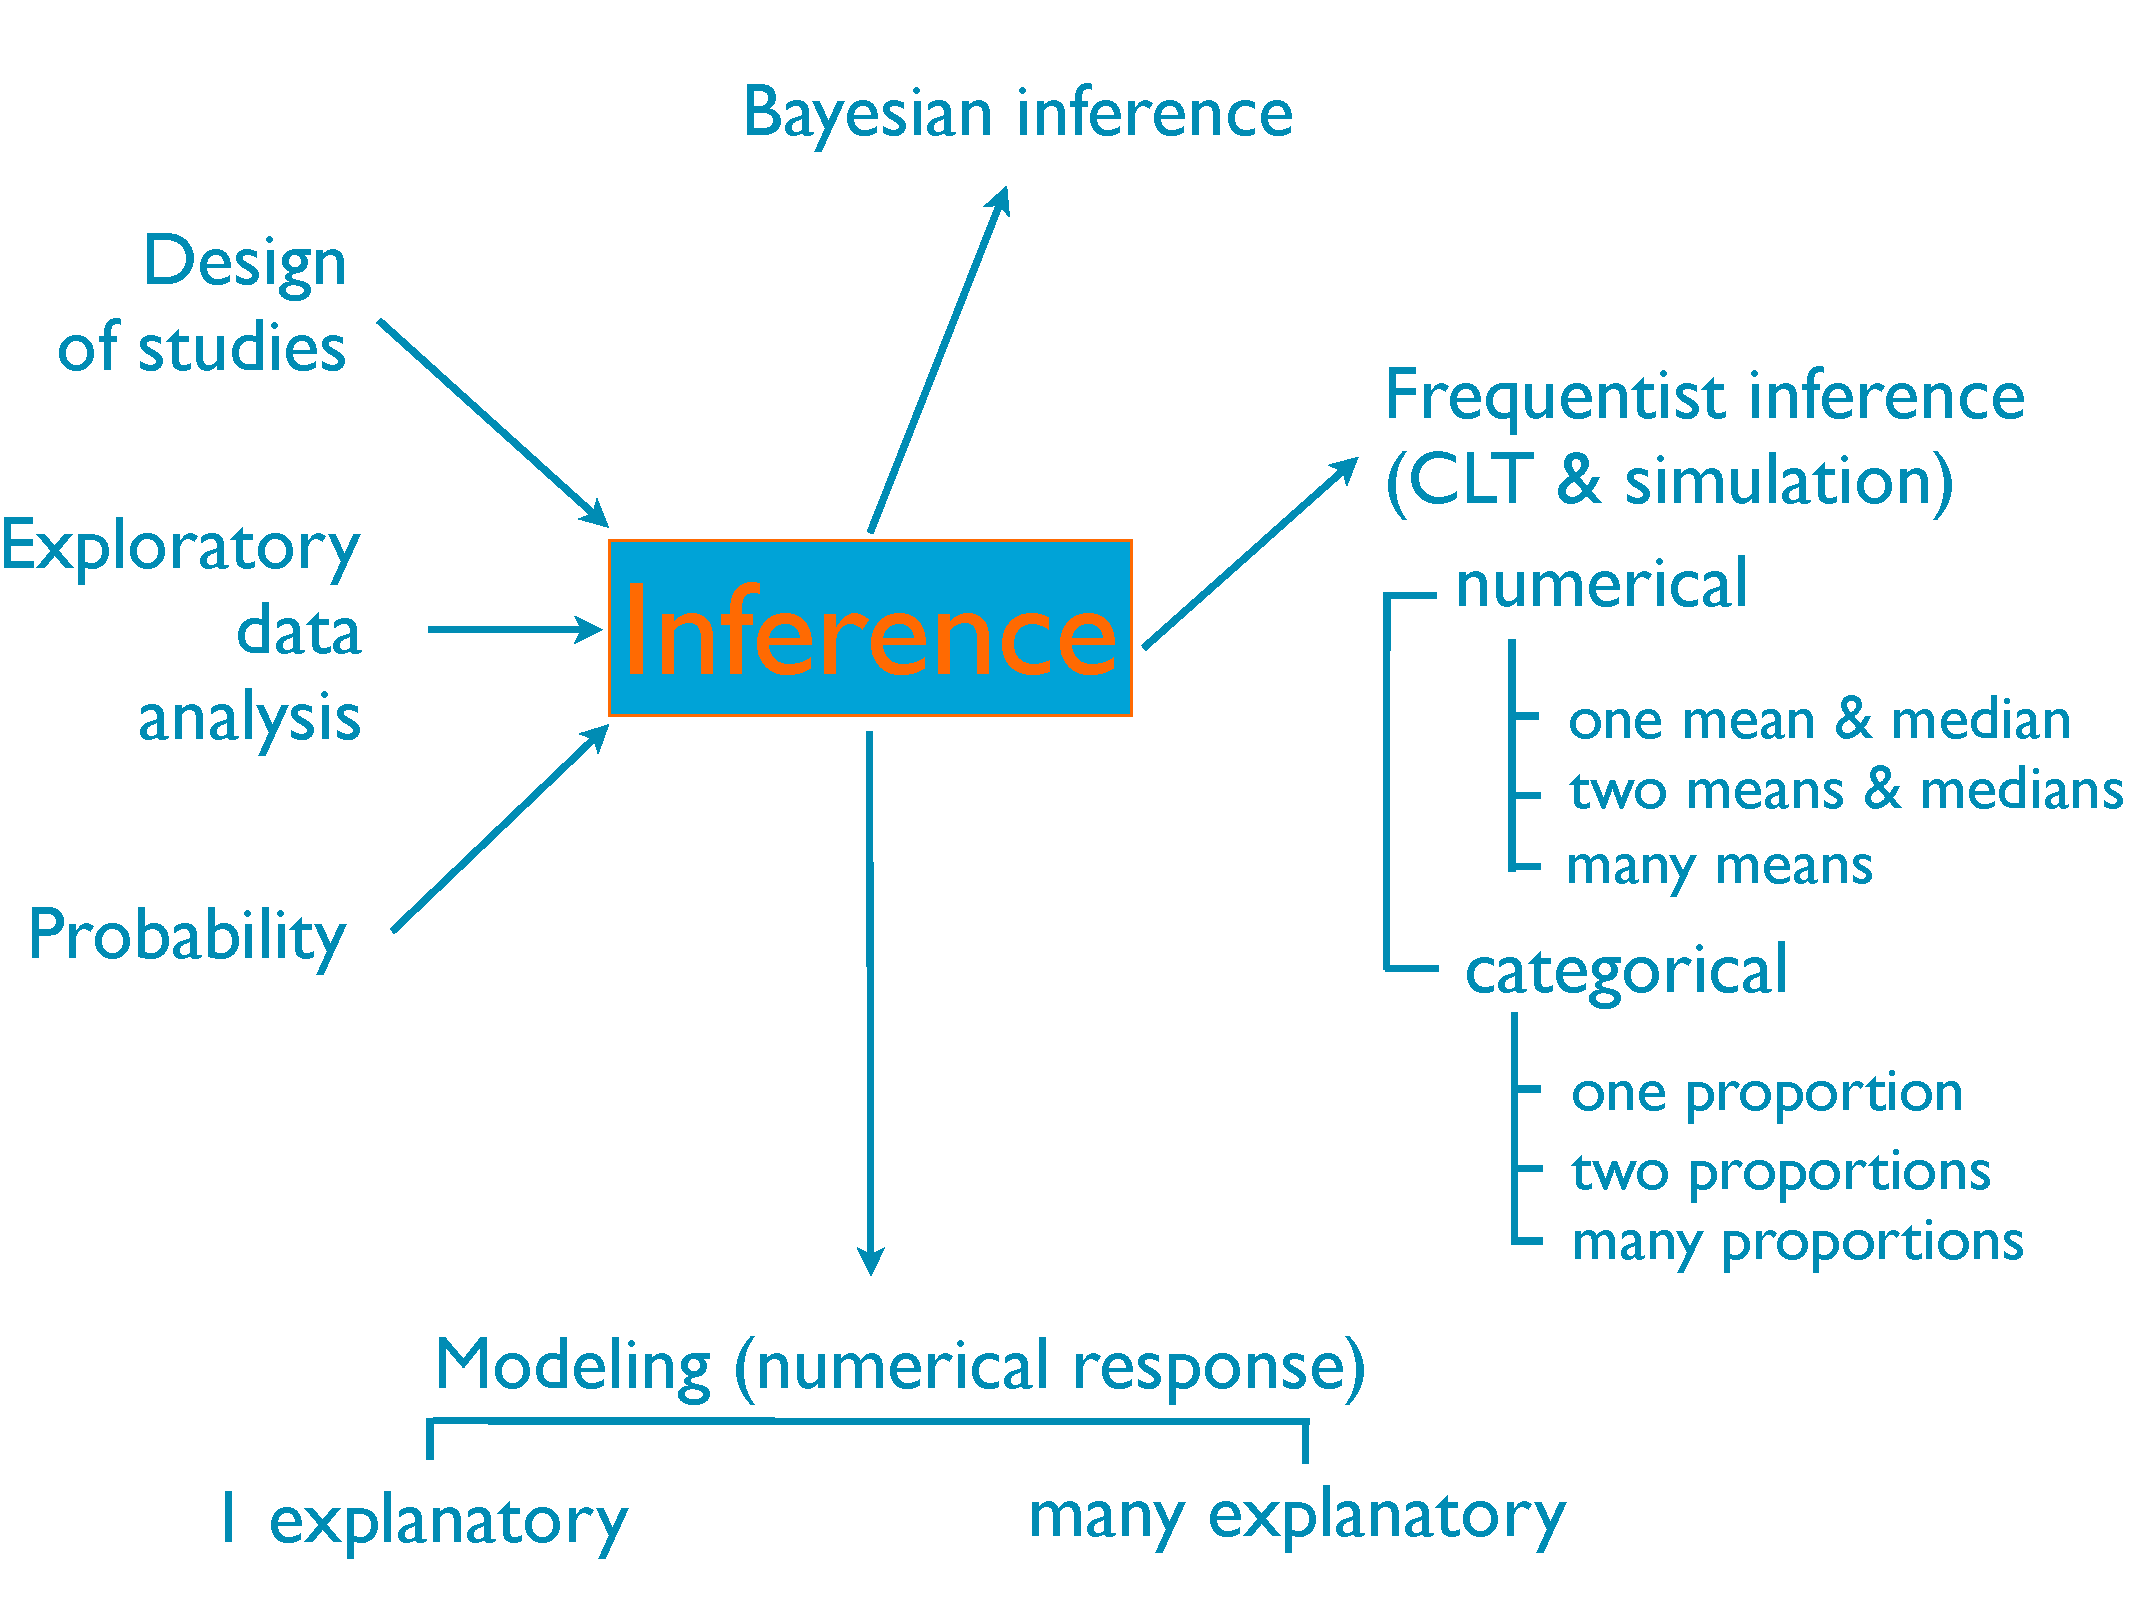
\includegraphics[width=\textwidth]{figures/map/inference}
}

\begin{enumerate}[(a)]
\item \solnMult{chi-square test of independence}
\item chi-square test of goodness of fit
\item anova
\item t-test
\end{enumerate}

\end{frame}

%%%%%%%%%%%%%%%%%%%%%%%%%%%%%%%%%%%%

\begin{frame}

\twocol{0.7}{0.3}
{
{\scriptsize
\clicker{Which of the following is the best method for evaluating the relationship between a numerical and a categorical variable with many levels?}}}
{
 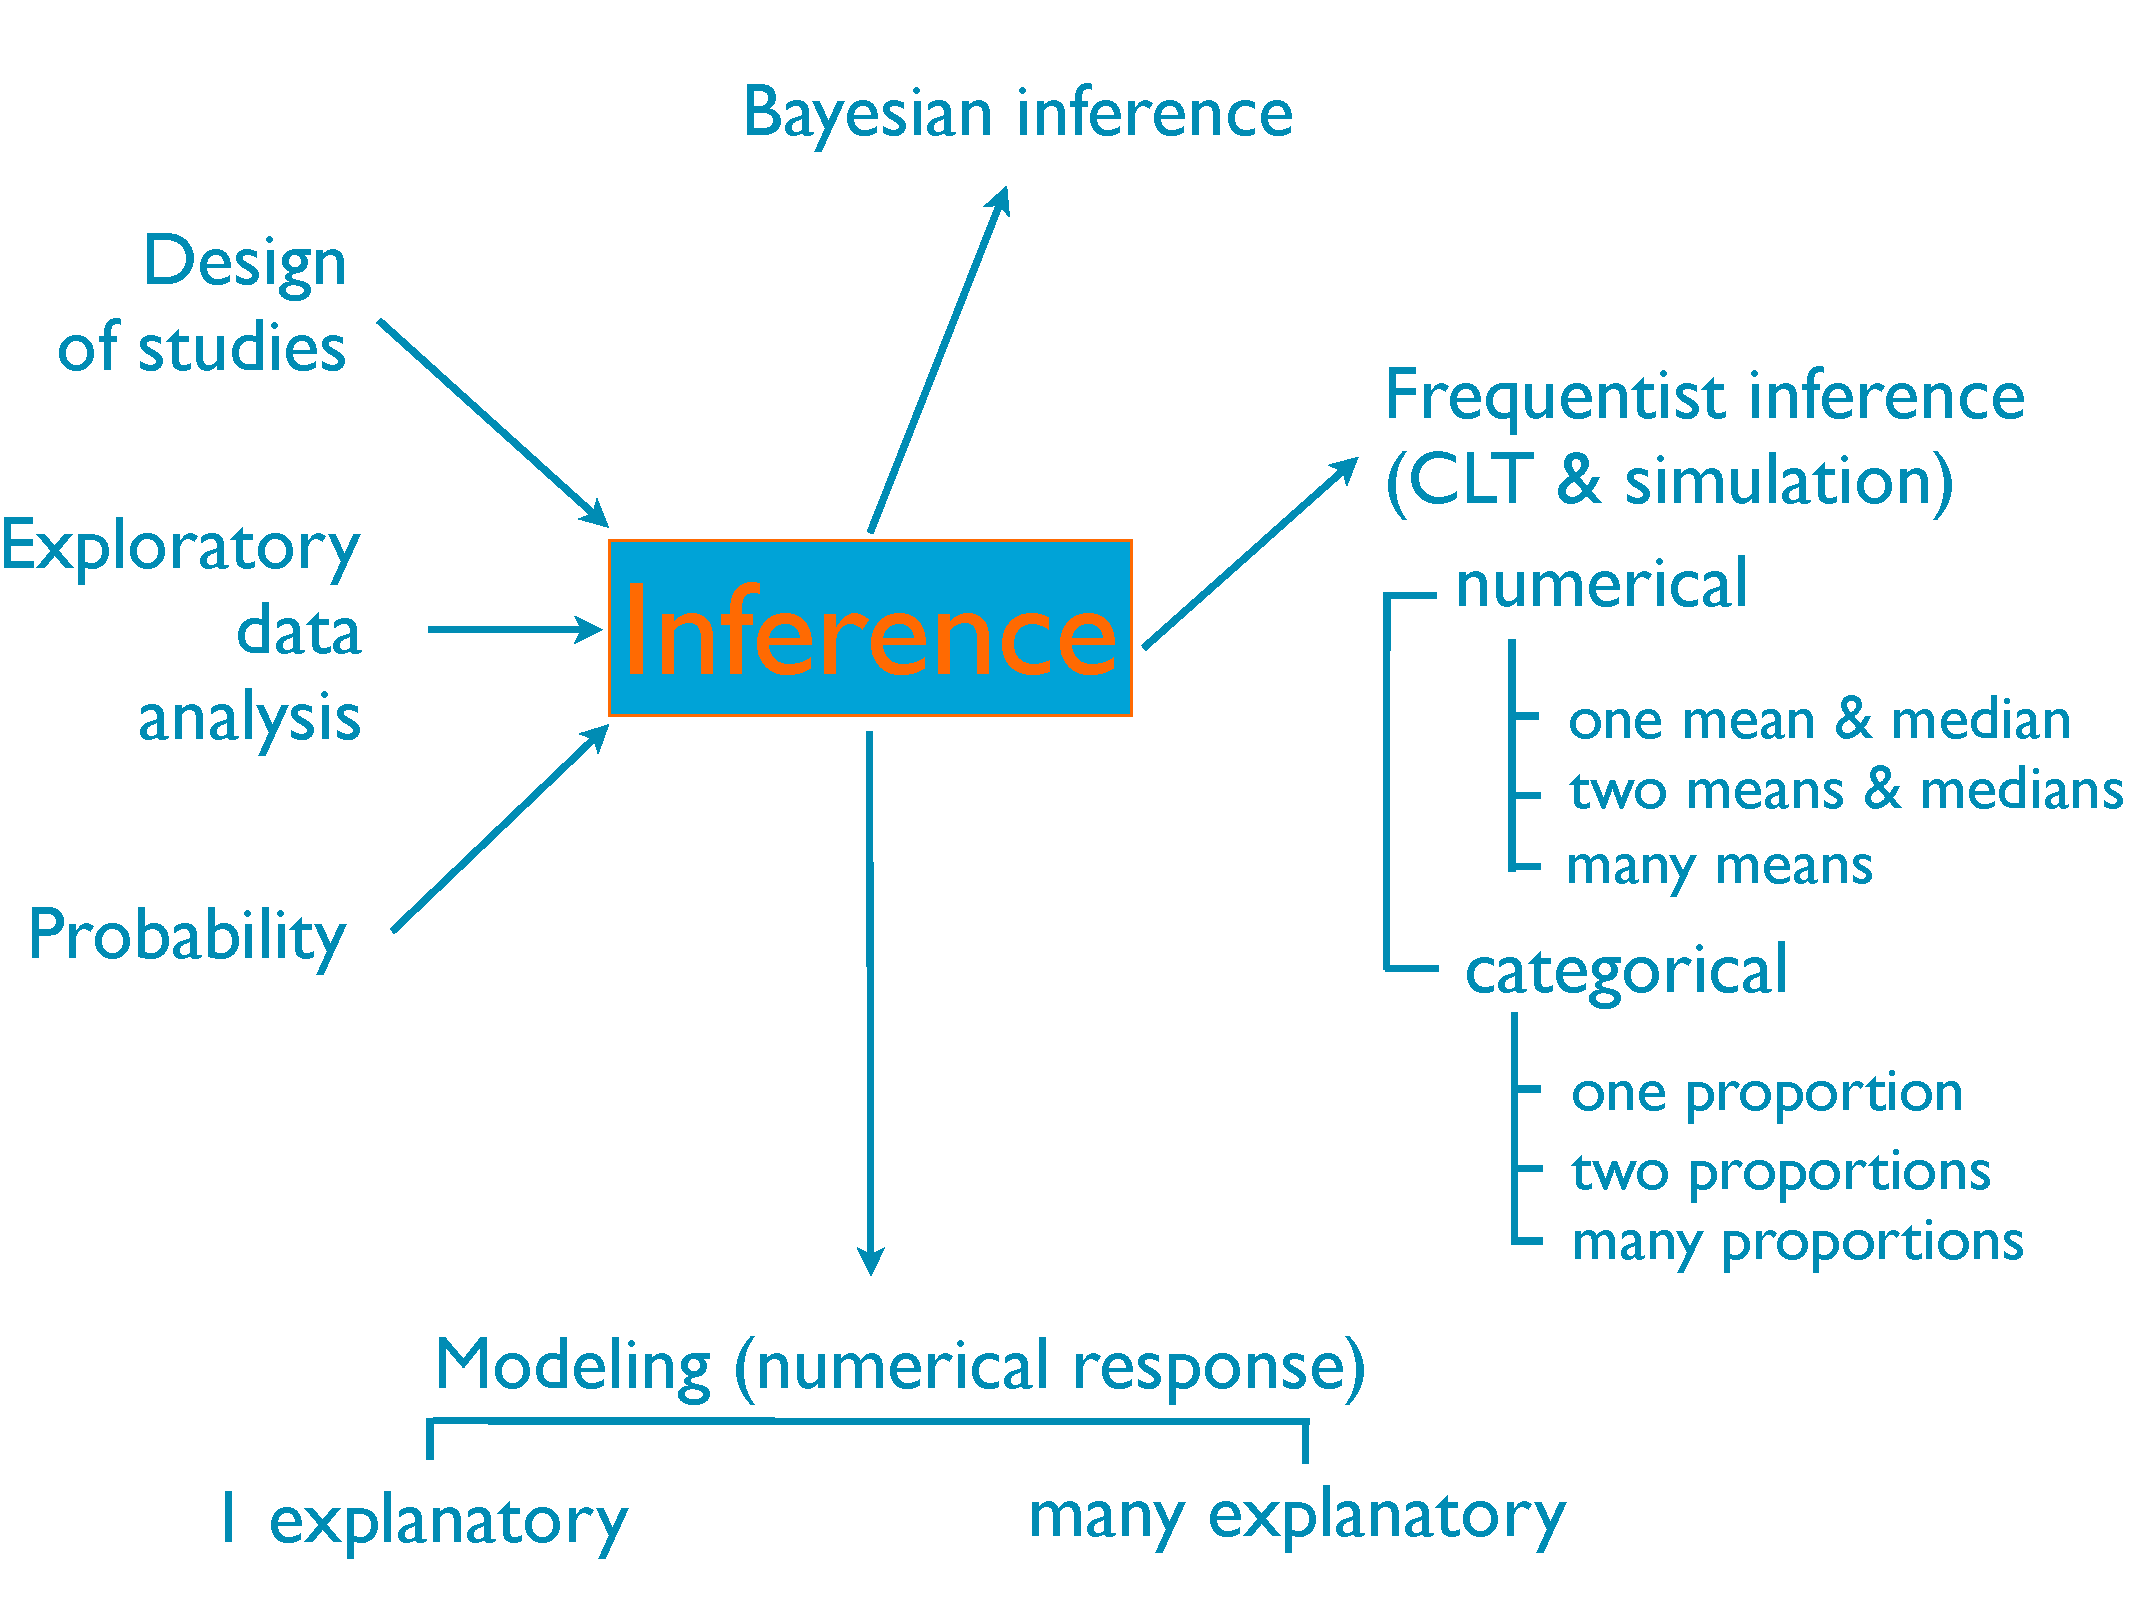
\includegraphics[width=\textwidth]{figures/map/inference}
}

\begin{enumerate}[(a)]
\item z-test
\item chi-square test of goodness of fit
\item \solnMult{ anova}
\item t-test
\end{enumerate}

\end{frame}

%%%%%%%%%%%%%%%%%%%%%%%%%%%%%%%%%%%%

\begin{frame}[fragile]

\twocol{0.7}{0.25}
{
{\scriptsize
\disc{Data are collected at a bank on 6 tellers' randomly sampled transactions. Do average transaction times vary by teller?}}}
{
 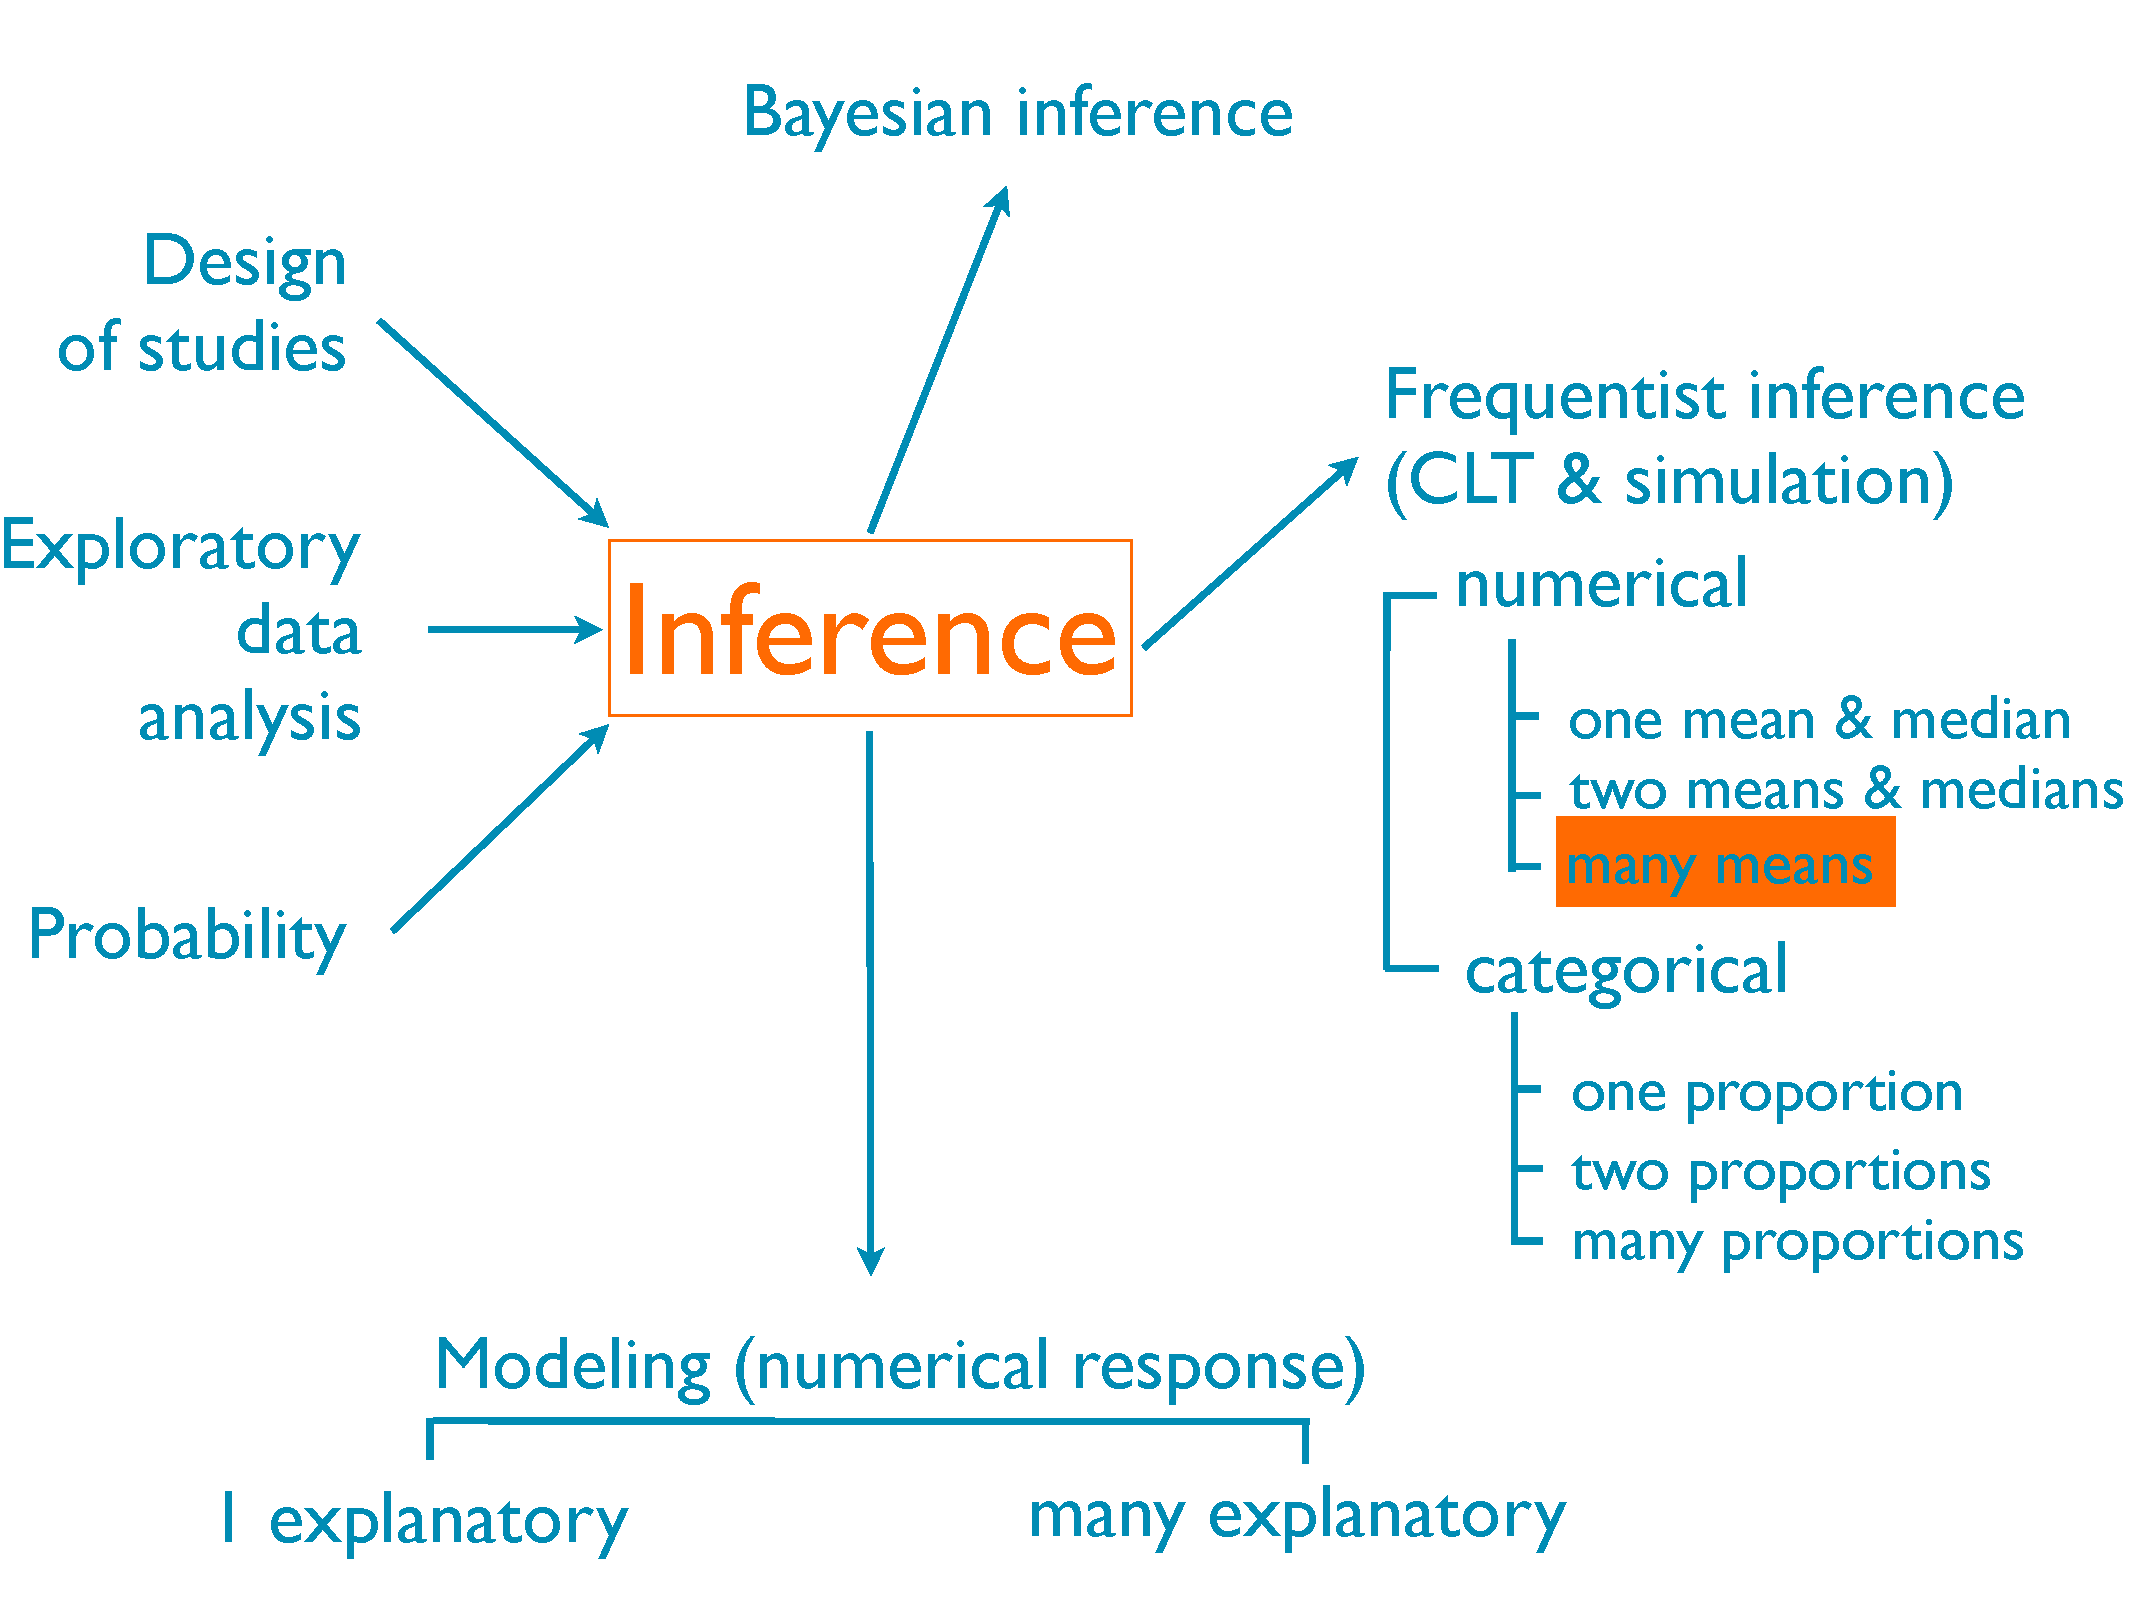
\includegraphics[width=\textwidth]{figures/map/many_mean}
}


{\scriptsize
\begin{verbatim}
Response variable: numerical, Explanatory variable: categorical
ANOVA

Summary statistics:
n_1 = 14, mean_1 = 65.7857, sd_1 = 15.2249
n_2 = 23, mean_2 = 79.9174, sd_2 = 23.284
n_3 = 15, mean_3 = 82.66, sd_3 = 18.1842
n_4 = 15, mean_4 = 77.9933, sd_4 = 23.2754
n_5 = 44, mean_5 = 81.7295, sd_5 = 21.5768
n_6 = 29, mean_6 = 75.3069, sd_6 = 20.4814

H_0: All means are equal.
H_A: At least one mean is different.
Analysis of Variance Table

Response: data
           Df Sum Sq Mean Sq F value Pr(>F)
group       5   3315  663.06   1.508 0.1914
Residuals 134  58919  439.69 
\end{verbatim}
}

\end{frame}

%%%%%%%%%%%%%%%%%%%%%%%%%%%%%%%%%%%%

\begin{frame}

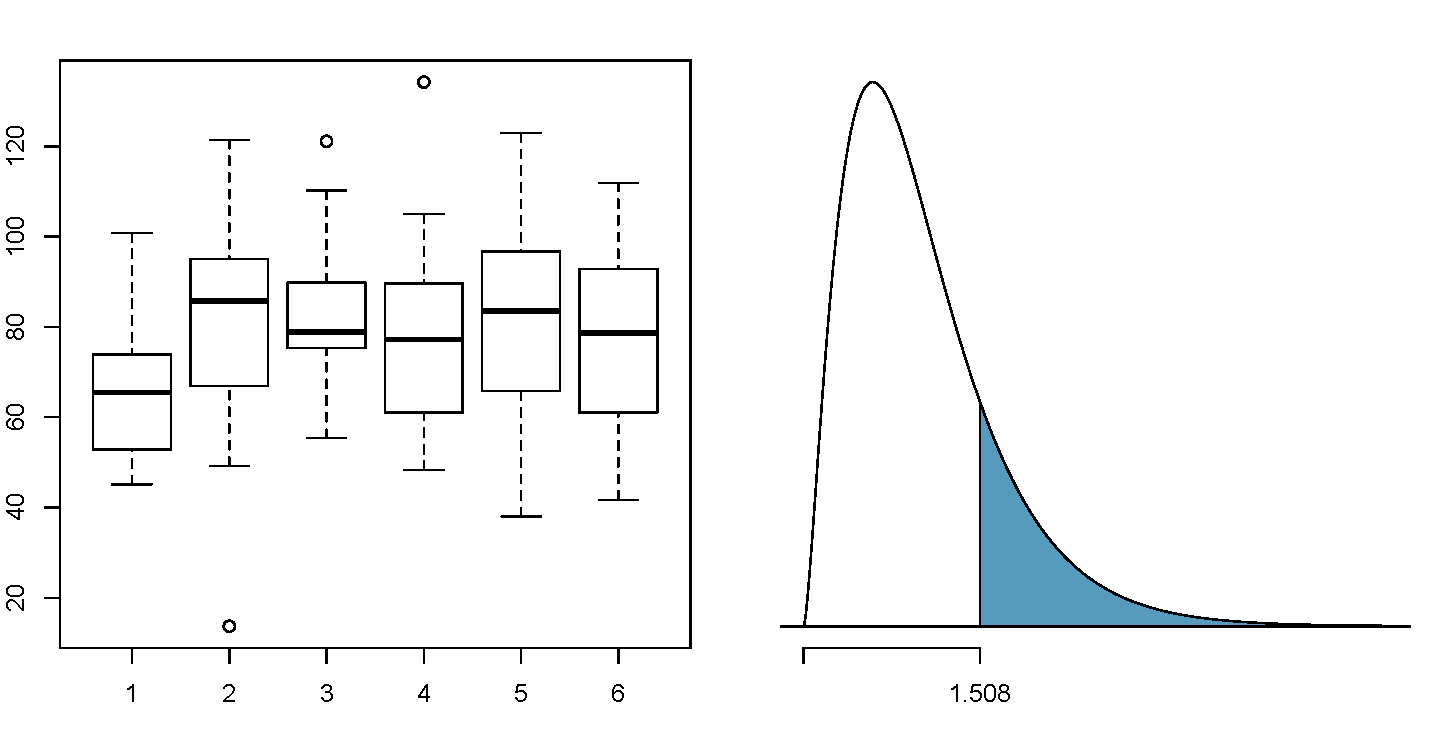
\includegraphics[width=\textwidth]{figures/anova/tellers}

\end{frame}

%%%%%%%%%%%%%%%%%%%%%%%%%%%%%%%%%%%%

\begin{frame}[fragile]

\twocol{0.7}{0.25}
{
{\scriptsize
\activity{}{Data are collected on download times at three different times during the day. We want to evaluate whether average download times vary by time of day. Fill in the ??s in the ANOVA output below.}}
}
{
 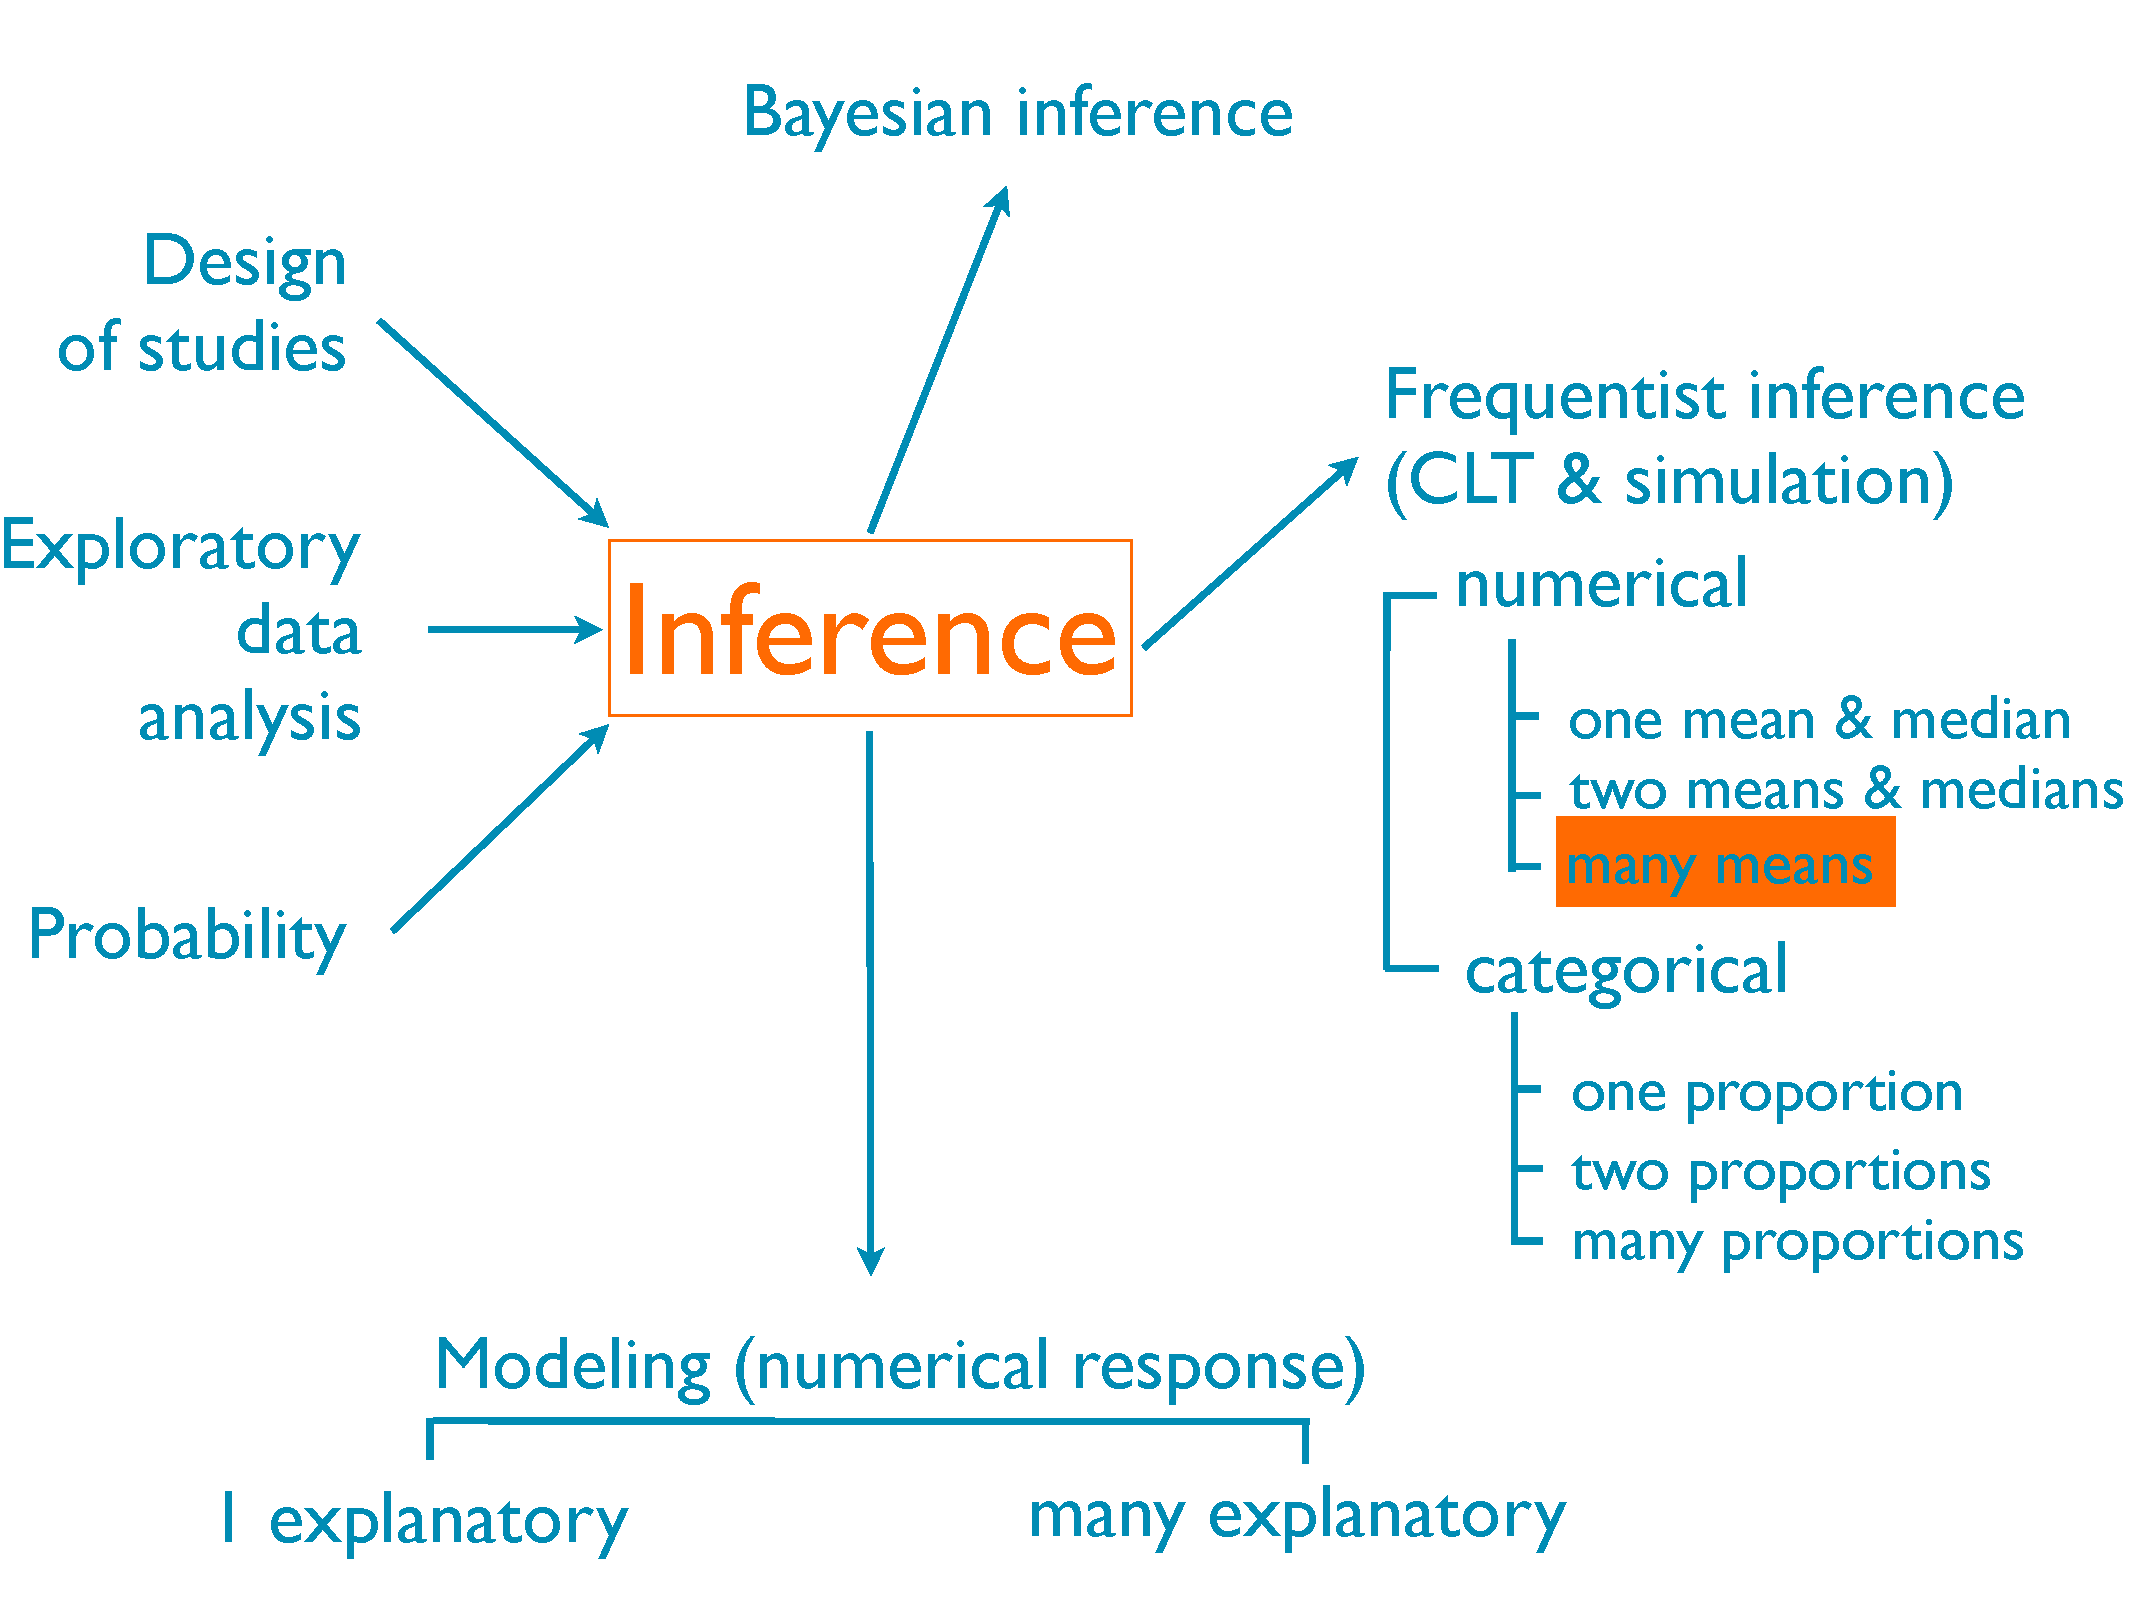
\includegraphics[width=\textwidth]{figures/map/many_mean}
}

{\scriptsize
\begin{verbatim}
Response variable: numerical, Explanatory variable: categorical
Summary statistics:
n_Early (7AM) = 16, mean_Early (7AM) = 113.375, sd_Early (7AM) = 47.6541
n_Eve (5 PM) = 16, mean_Eve (5 PM) = 273.3125, sd_Eve (5 PM) = 52.1929
n_Late (12 AM) = 16, mean_Late (12 AM) = 193.0625, sd_Late (12 AM) = 40.9023
\end{verbatim}
}

{\small
\begin{verbatim}
Analysis of Variance Table
Response: data
          Df Sum Sq Mean Sq F value    Pr(>F)
group     ??     ??      ??      ?? 1.306e-11
Residuals ?? 100020      ??        
Total     ?? 304661  
\end{verbatim}
}

\end{frame}

%%%%%%%%%%%%%%%%%%%%%%%%%%%%%%%%%%%%

\begin{frame}

\disc{What is the result of the ANOVA?}

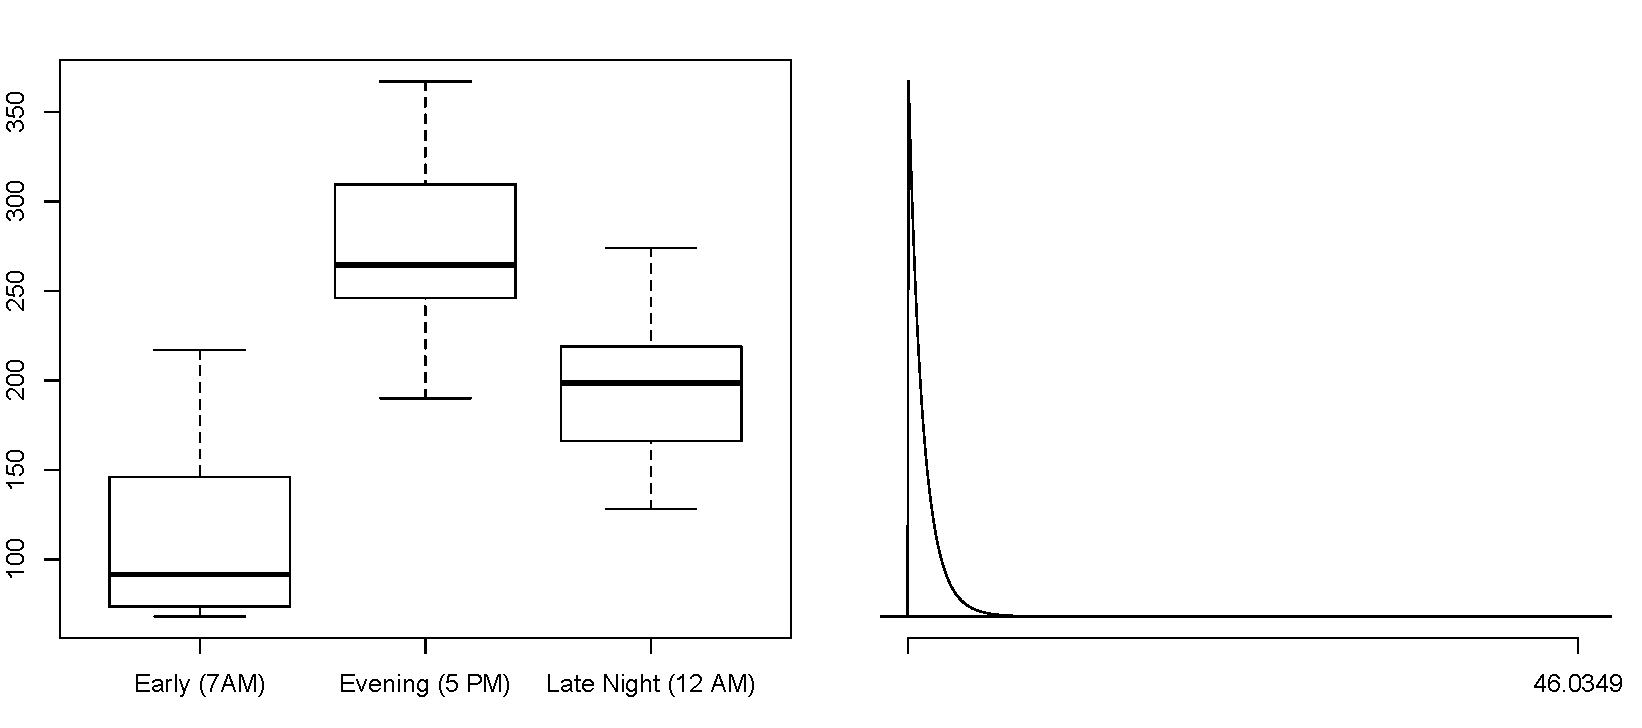
\includegraphics[width=\textwidth]{figures/anova/dl}

\pause

\soln{Since 1.306e-11 $<$ 0.05, we reject the null hypothesis. The data provide convincing evidence that the  average download time is different for at least one pair of times of day.}

\end{frame}

%%%%%%%%%%%%%%%%%%%%%%%%%%%%%%%%%%%%

\begin{frame}

\activity{}{The next step is to evaluate the pairwise tests. There are 3 pairs of times of day
\begin{enumerate}
\item Early vs. Evening: left side of class (facing the board)
\item Evening vs. Late Night: center of class
\item Early vs. Late Night: right side of class
\end{enumerate}
Determine the appropriate significance level for these tests, and then complete the test assigned to your team.
}

\end{frame}

%%%%%%%%%%%%%%%%%%%%%%%%%%%%%%%%%%%%

\begin{frame}

\soln{$\alpha^\star = 0.05 / 3 = 0.0167$}

\pause

\soln{
{\scriptsize
\begin{columns}
\column{0.33\textwidth}
(1) Early vs. Evening
\pause
\begin{eqnarray*}
T_{45} &=& \frac{113.375 - 273.3125}{\sqrt{\frac{2223}{16} + \frac{2223}{16}}} \\
\pause
&=& \frac{-159.9375}{16.67} =  -9.59 \\
\pause
&&p-val < 0.01
\end{eqnarray*}
\pause
\column{0.33\textwidth}
(2) Evening vs. Late Night 
\pause
\begin{eqnarray*}
T_{45} &=& \frac{113.375 - 193.0625}{\sqrt{\frac{2223}{16} + \frac{2223}{16}}} \\
\pause
&=& \frac{-79.6875}{16.67} =  -4.78 \\
\pause
&&p-val < 0.01
\end{eqnarray*}
\pause
\column{0.33\textwidth}
(3) Early vs. Late Night  
\pause
\begin{eqnarray*}
T_{45} &=& \frac{273.3125 - 193.0625}{\sqrt{\frac{2223}{16} + \frac{2223}{16}}} \\
\pause
&=& \frac{80.25}{16.67} =  4.81 \\
\pause
&&p-val < 0.01
\end{eqnarray*}
\end{columns}
}}

\end{frame}

%%%%%%%%%%%%%%%%%%%%%%%%%%%%%%%%%%%%

\begin{frame}[fragile]

\twocol{0.7}{0.25}
{
{\scriptsize
\clicker{What percent of variability in download times is explained by time of day?}}}
{
 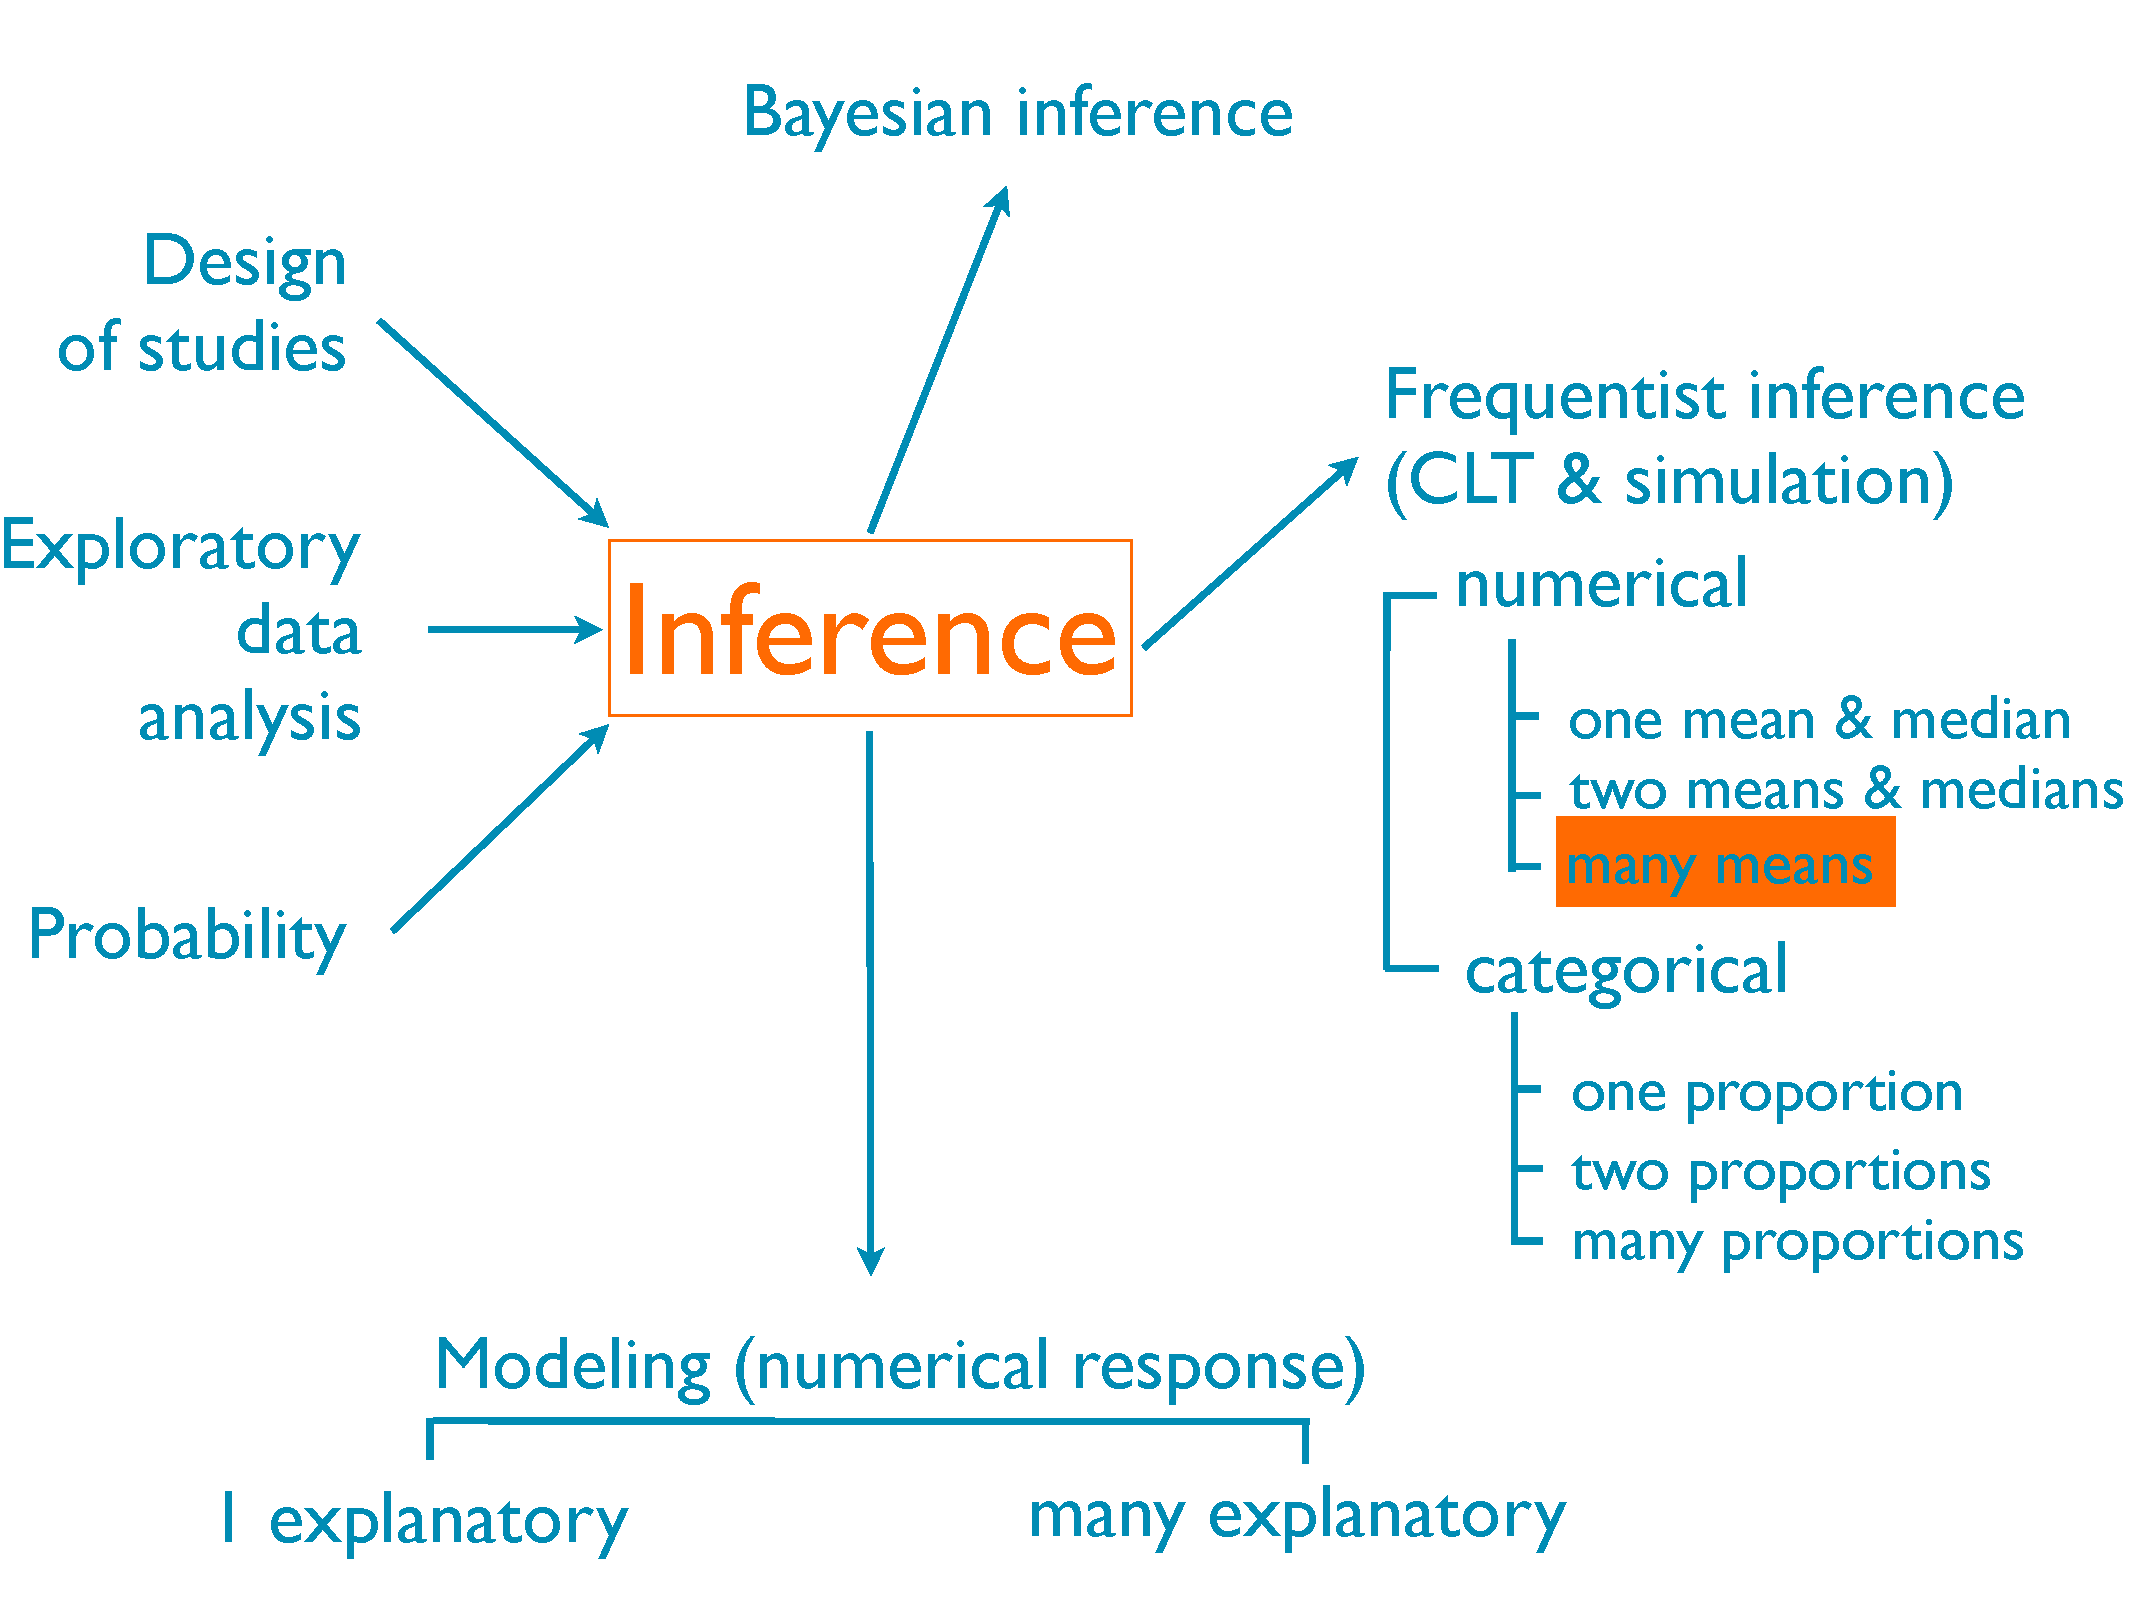
\includegraphics[width=\textwidth]{figures/map/many_mean}
}

{\scriptsize
\begin{verbatim}
Response: data
          Df Sum Sq Mean Sq F value    Pr(>F)
group      2 204641  102320  46.035 1.306e-11
Residuals 45 100020    2223                  
\end{verbatim}
}

\begin{enumerate}[(a)]
\item \solnMult{ $\frac{204641}{204641 + 100020}$ } \soln{\only<2>{\red{ = 0.67}}}
\item $\frac{204641}{100020}$
\item $\frac{100020}{204641}$
\item $\frac{102320}{102320 + 2223}$
\end{enumerate}

\end{frame}

%%%%%%%%%%%%%%%%%%%%%%%%%%%%%%%%%%%%

\begin{frame}

\twocol{0.7}{0.3}
{
{\scriptsize
\clicker{$n = 50$ and $\hat{p} = 0.80$. Hypotheses: $H_0: p = 0.82; H_A: p \ne 0.82$. We use a randomization test because the sample size isn't large enough for $\hat{p}$ to be distributed nearly normally ($50 \times 0.82 = 41 < 10; 50 \times 0.18 = 9 < 10$). Which of the following is the correct set up for this hypothesis test? Red: success, blue: failure, $\hat{p}_{sim}$ = proportion of reds in simulated samples.
}}}
{
 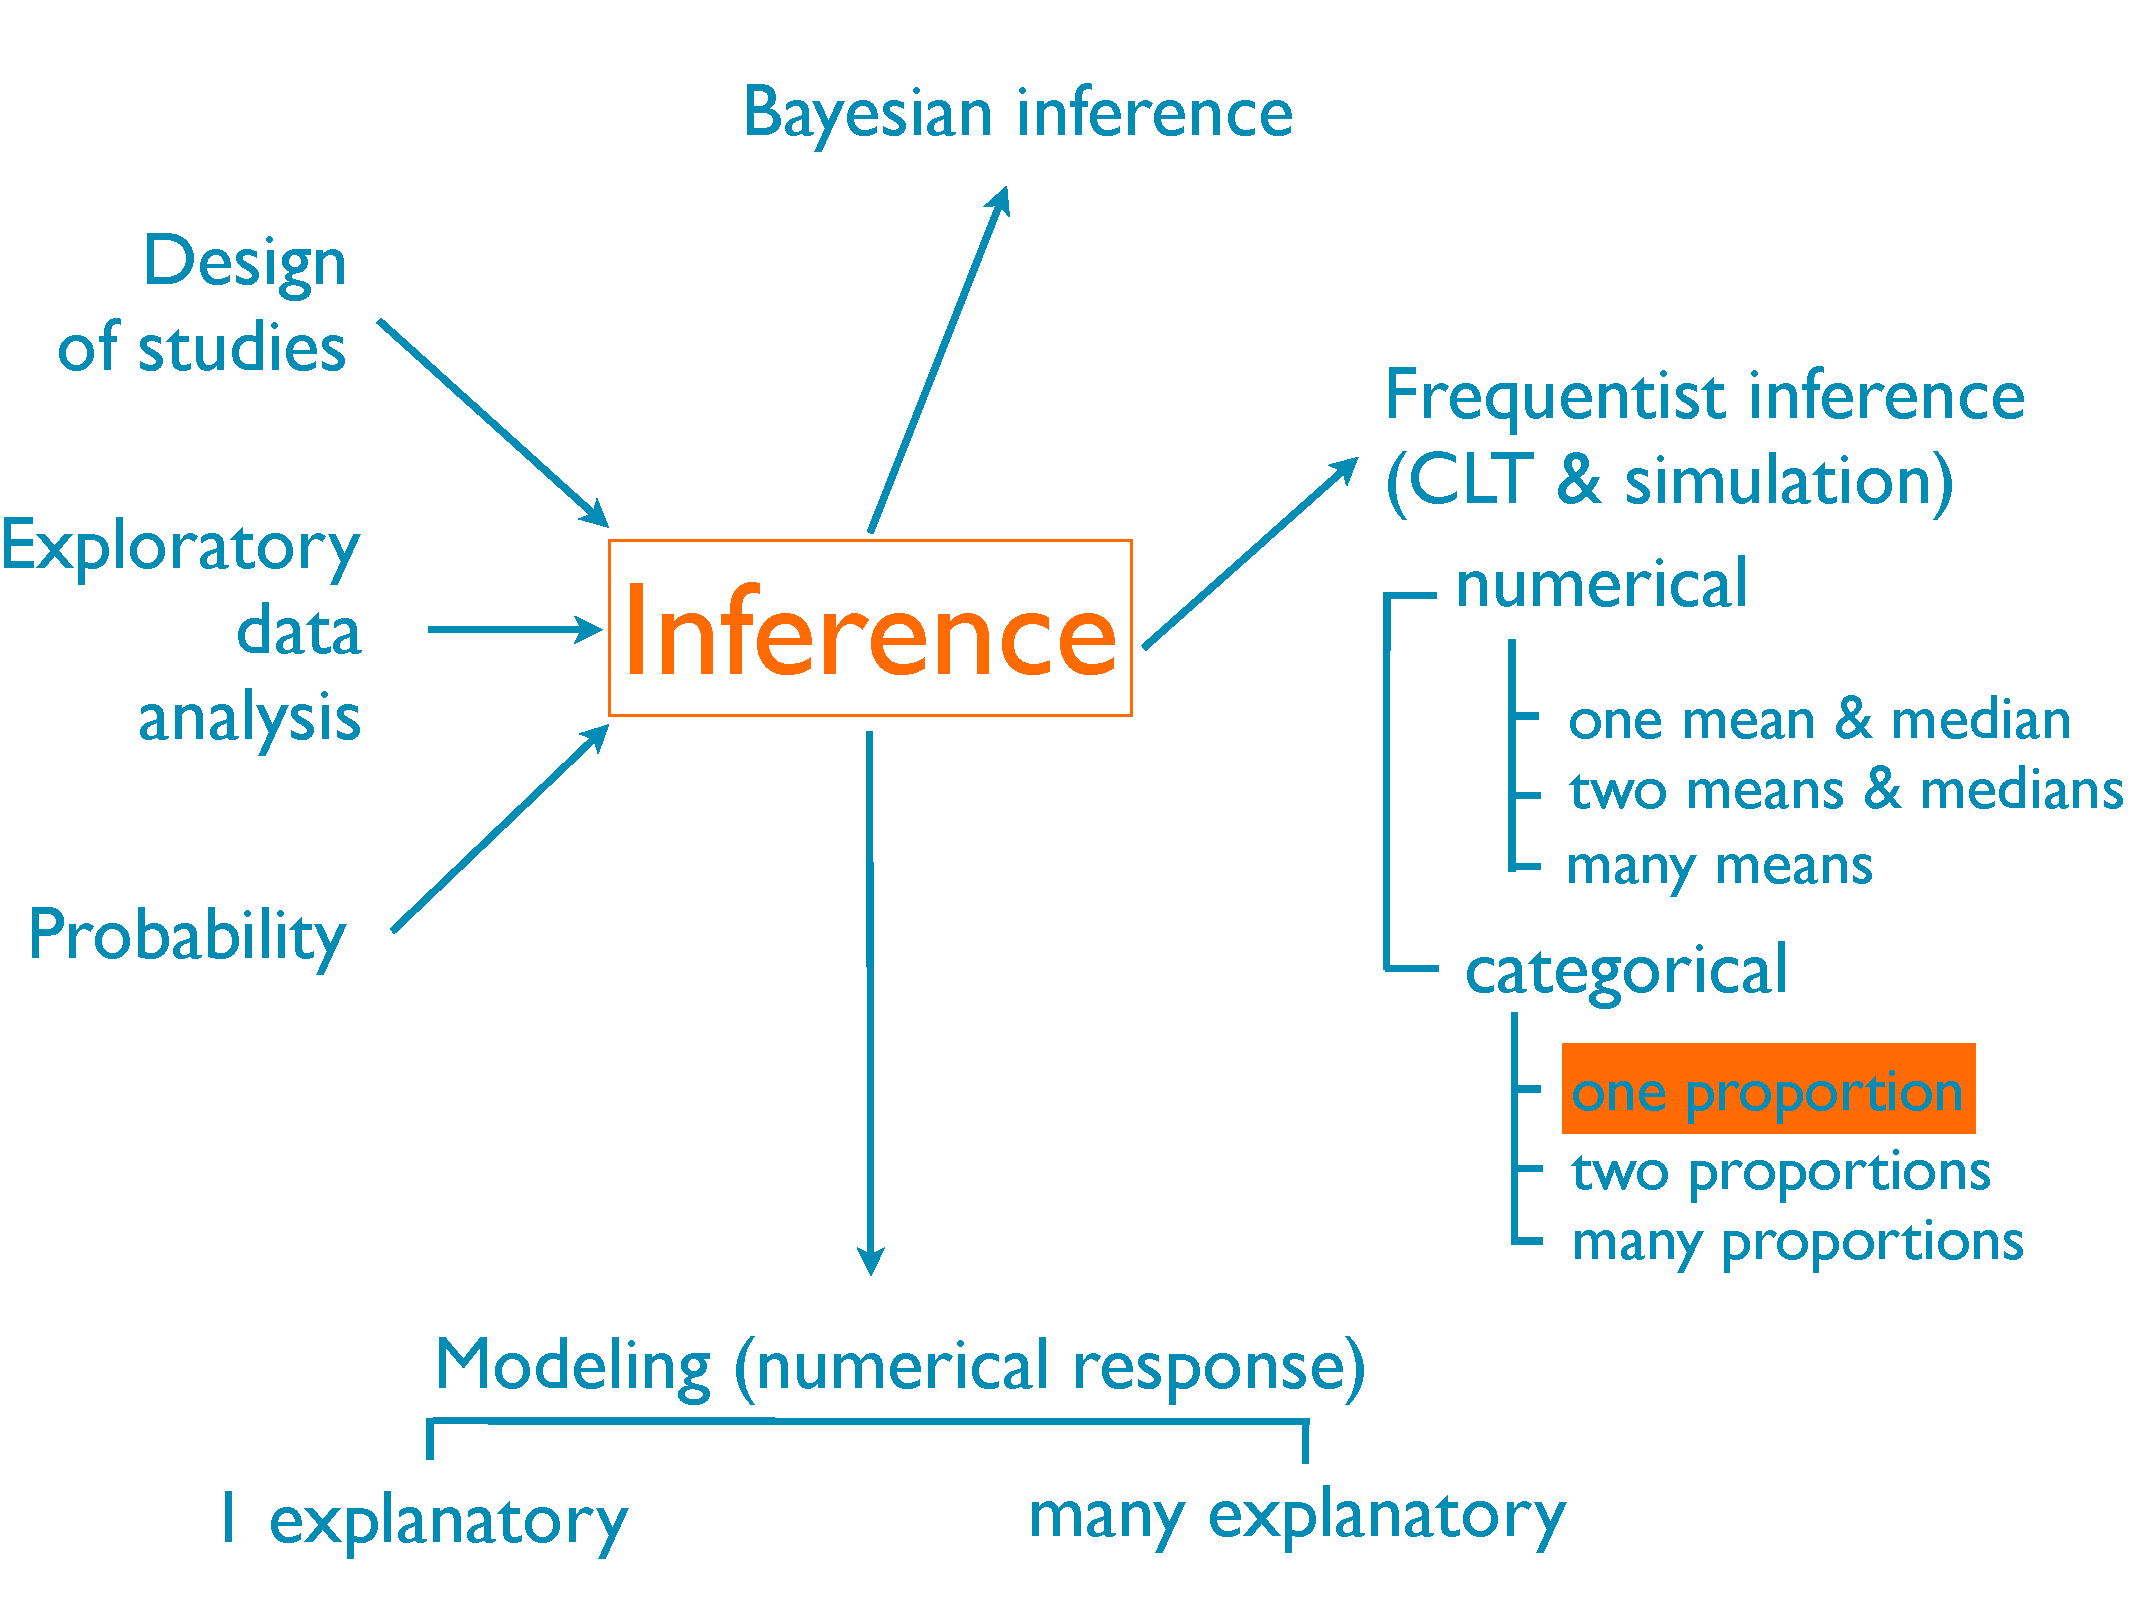
\includegraphics[width=\textwidth]{figures/map/one_prop}
}

\vfill

{\footnotesize
\begin{enumerate}[(a)]
\item Place 80 red and 20 blue chips in a bag. Sample, \underline{with} replacement, 50 chips and calculate the proportion of reds. Repeat this many times and calculate the proportion of simulations where $\hat{p}_{sim} \ne 0.82$. 
\item Place 82 red and 18 blue chips in a bag. Sample, \underline{without} replacement, 50 chips and calculate the proportion of reds. Repeat this many times and calculate the proportion of simulations where $\hat{p}_{sim} \ne 0.80$.
\item \solnMult{Place 82 red and 18 blue chips in a bag. Sample, \underline{with} replacement, 50 chips and calculate the proportion of reds. Repeat this many times and calculate the proportion of simulations where $\hat{p}_{sim} \le 0.80$ or $\hat{p}_{sim} \ge 0.84$.}
\item Place 82 red and 18 blue chips in a bag. Sample, \underline{with} replacement, 100 chips and calculate the proportion of reds. Repeat this many times and calculate the proportion of simulations where $\hat{p}_{sim} \le 0.80$ or $\hat{p}_{sim} \ge 0.84$. 
\end{enumerate}
}

\end{frame}

%%%%%%%%%%%%%%%%%%%%%%%%%%%%%%%%%%%%

\begin{frame}

\disc{What is / should be the center of the randomization distribution? What is the result of the hypothesis test?}

\begin{center}
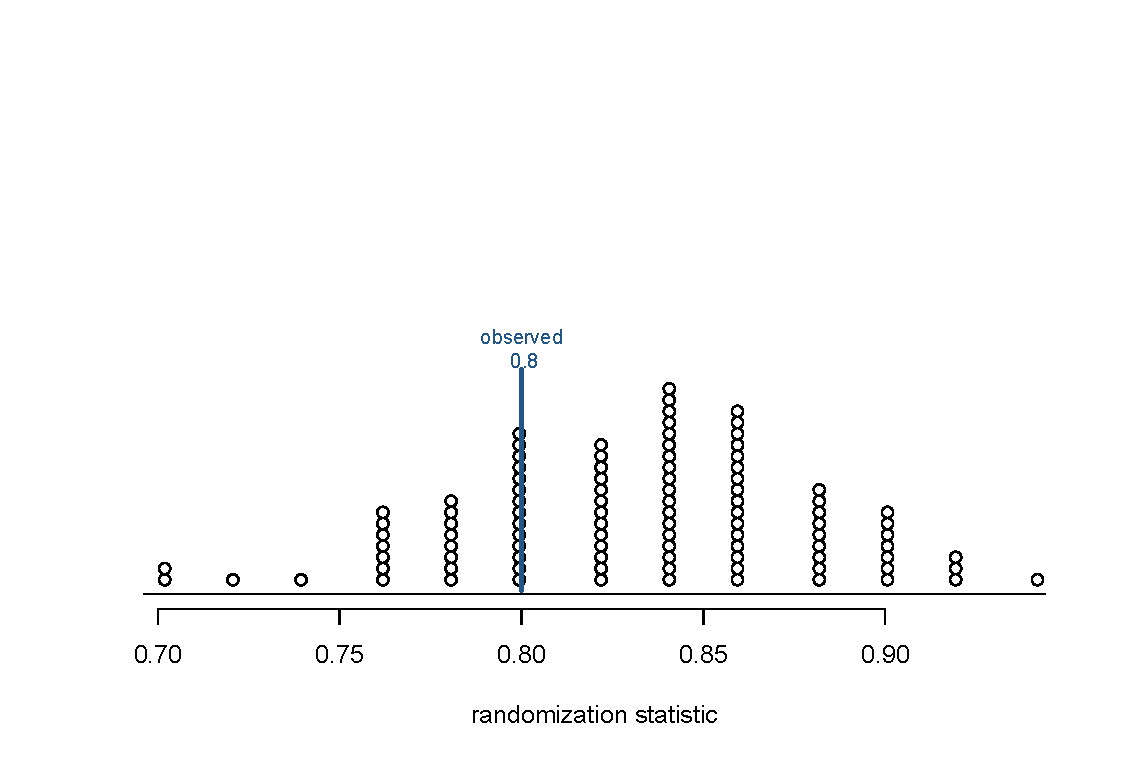
\includegraphics[width=\textwidth]{figures/rand_dist}
\end{center}

\end{frame}

%%%%%%%%%%%%%%%%%%%%%%%%%%%%%%%%%%%%

\section{Summary of methods}

%%%%%%%%%%%%%%%%%%%%%%%%%%%%%%%%%%%%

\begin{frame}
\frametitle{Inference for numerical data:}

\pause

\begin{itemize}

\item One numerical: \\
\begin{itemize}
\item Parameter of interest: $\mu$
\item $T$
\item HT and CI
\end{itemize}

\pause

\item One numerical vs. one categorical (with 2 levels):
\begin{itemize}
\item Parameter of interest: $\mu_1 - \mu_2$
\item $T$
\item HT and CI
\pause
\item If samples are dependent (paired), first find differences between paired observations
\end{itemize}

\pause

\item One numerical vs. one categorical (with $3+$ levels) - mean: \\
\begin{itemize}
\item Parameter of interest: N/A
\item ANOVA
\item HT only
\end{itemize}

\pause

\item For all other parameters of interest: simulation

\end{itemize}

\end{frame}

%%%%%%%%%%%%%%%%%%%%%%%%%%%%%%%%%%%%

\begin{frame}
\frametitle{Inference for categorical data - binary outcome:}

\textbf{Binary outcome:}

\pause

\begin{itemize}

\item One categorical: \\
\begin{itemize}
\item Parameter of interest: $p$
\item S/F condition met $\rightarrow$ Z, if not simulation
\item HT and CI
\end{itemize}

\pause

\item One categorical vs. one categorical, each with only 2 outcomes: \\
\begin{itemize}
\item Parameter of interest: $p_1 - p_2$
\item S/F condition met $\rightarrow$ Z, if not simulation
\item HT and CI
\end{itemize}

\pause

\item S/F: use observed S and F for CIs and expexted for HT

\end{itemize}

\end{frame}

%%%%%%%%%%%%%%%%%%%%%%%%%%%%%%%%%%%%

\begin{frame}
\frametitle{Inference for categorical data - $3+$ outcomes:}

\textbf{$3+$ outcomes:}

\pause

\begin{itemize}

\item One categorical, compared to hypothetical distribution: \\
\begin{itemize}
\item Parameter of interest: N/A
\item At least 5 expected  successes in each cell $\rightarrow$ $\chi^2$ GOF, if not simulation
\item HT only
\end{itemize}

\pause

\item One categorical vs. one categorical, either with $3+$ outcomes: \\
\begin{itemize}
\item Parameter of interest: N/A
\item At least 5 expected successes in each cell $\rightarrow$ $\chi^2$ Independence, if not simulation
\item HT only
\end{itemize}

\end{itemize}

\end{frame}

%%%%%%%%%%%%%%%%%%%%%%%%%%%%%%%%%%%%

\end{document}